%!TEX root = ../main.tex
%=========================================================

\section{Performance Evaluation}
\label{sec:eval}

We evaluate \sysname first with two complementary means: an actual implementation and large-scale simulations.

\subsection{Prototype}

We implemented \sysname in the \emph{Go Ethereum} (Geth) client~\cite{geth} and made it fully compliant with the Ethereum P2P protocol suite. 
We perform our initial tests on a single testbed with 24 cores AMD Ryzen Threadripper 3960X CPU and 256GB of RAM.
We launch 1,000 nodes using IDs/IP addressed randomly drafted from the Ethereum live network~\cite{discv4-dns-lists} and 20 topics following the distribution perceived in \Cref{fig:ecosystem}.
Each node constantly register for the assigned topic and performs 5 lookup operations, aiming to discover $N_\textit{lookup}=30$ peers.

We first analyze the average number of lookup results obtained by each node. 
\Cref{fig:testbed_discovered_search} groups nodes by the topic they participate in, as indicated by the colors of the bars (order within one color is random).
Topics are sorted from highest to lowest popularity, as can be seen by the width of the color zones.
The vast majority of nodes is always able to find the required number of peers.
Less popular topic nodes (right side of the graph) do not always obtain enough results.
This is caused by the lower number of participants for those topics ($< 30$).
Importantly, within each topic, we observe the same number of obtained results indicating high fairness.
Every node in the network is able to efficiently find its peers.

\begin{figure}
\centering
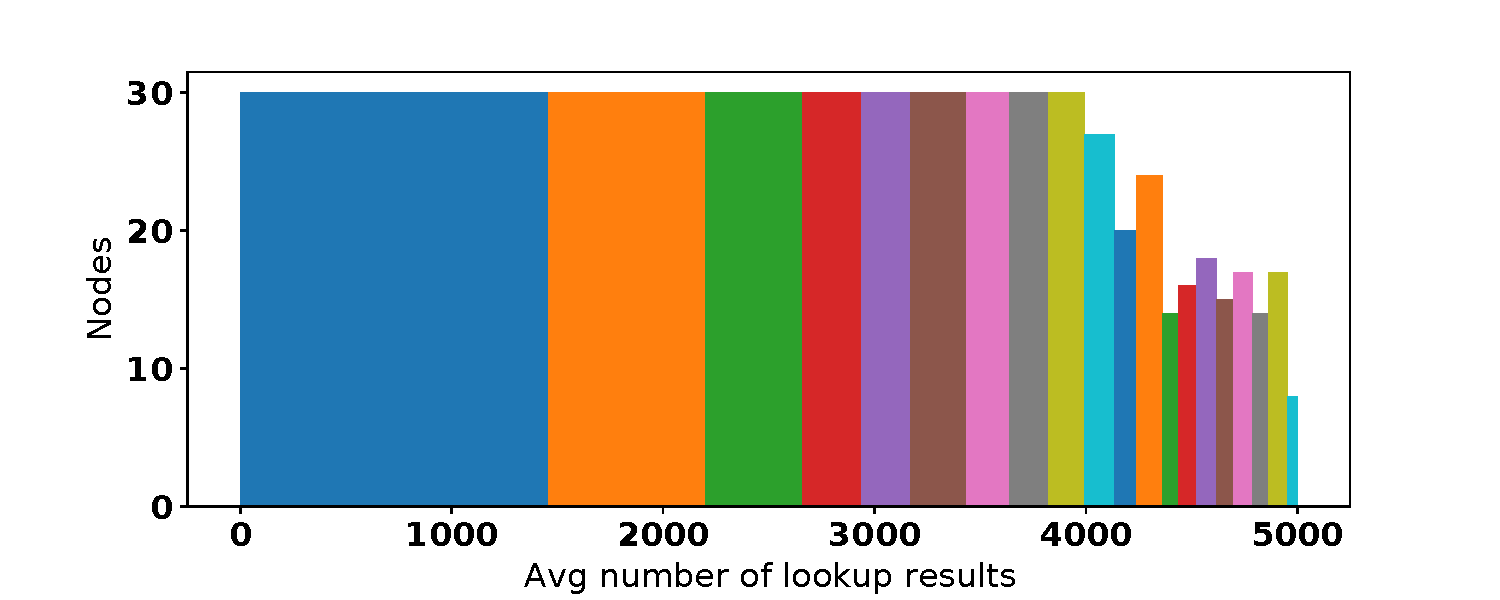
\includegraphics[width=\linewidth]{results/testbed/testbed_discovered_search.pdf}
\caption{\label{fig:testbed_discovered_search}Average number of lookup results obtained by each node.}
\vspace{-0.15in}
\end{figure}

\begin{figure}
\centering
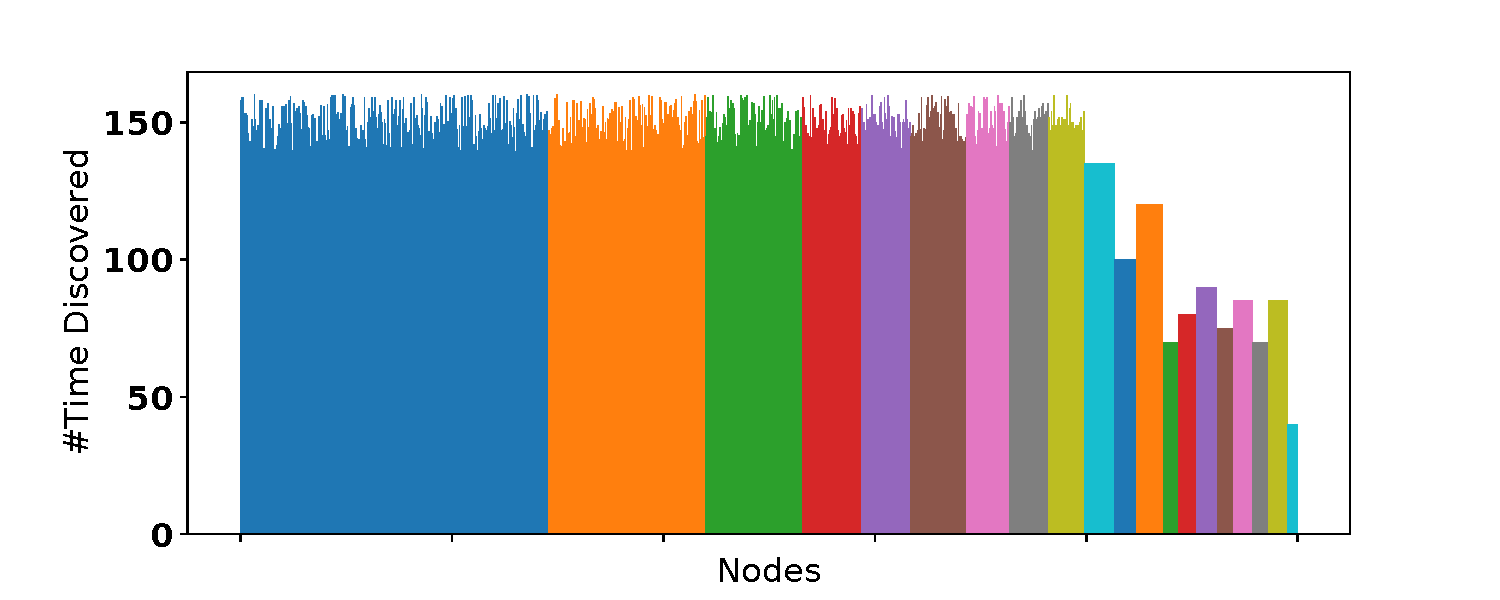
\includegraphics[width=\linewidth]{results/testbed/testbed_times_discovered.pdf}
\caption{\label{fig:testbed_time_discovered}Number of times each node is discovered during lookup.}
\vspace{-0.15in}
\end{figure}

\Cref{fig:testbed_time_discovered} presents the number of time each node is discovered by others. 
It allows us to verify that no node is discriminated in the network.
We use the same visual grouping as in \Cref{fig:testbed_discovered_search}.
Within each topic, nodes are discovered a very similar amount of times as peers from the same topic, and we did not observe nodes that would not be discovered by their peers. 
The distribution closely matches the one observed in \Cref{fig:testbed_discovered_search}. 

The results indicate the \sysname lookup process is a sound basis to spawn a healthy, application-specific p2p network regardless of the application popularity.

At first, the equal discovery rate across topics with different popularity might be surprising.
To investigate it further, for each topic, we plot the average total waiting time received by its advertisers.
We express the waiting time in ad lifetimes $a$ and keep the topic colors consistent with the one used in \Cref{fig:testbed_time_discovered} and \Cref{fig:testbed_time_discovered}.
The waiting time function returns higher waiting times to nodes from popular applications.
As a result, those nodes will spend less time in the ad caches and more time waiting to be admitted.
This mechanism allows advertisements of less popular topics to get a fair share of ad cache space and results in an equal discovery rate presented above. 

\begin{figure}
\centering
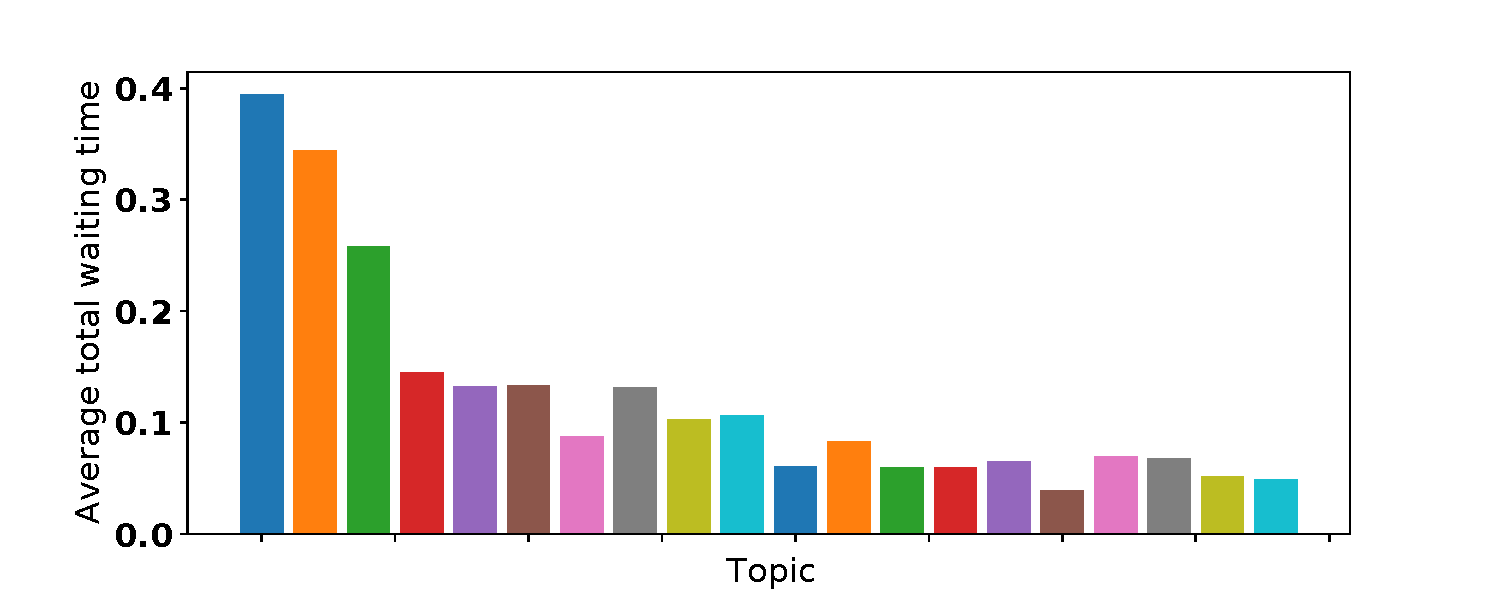
\includegraphics[width=\linewidth]{results/testbed/waiting_time.pdf}
\caption{Average total waiting times received per topic.}
\label{fig:testbed_waiting_time}
\vspace{-0.15in}
\end{figure}

\begin{figure}
\centering
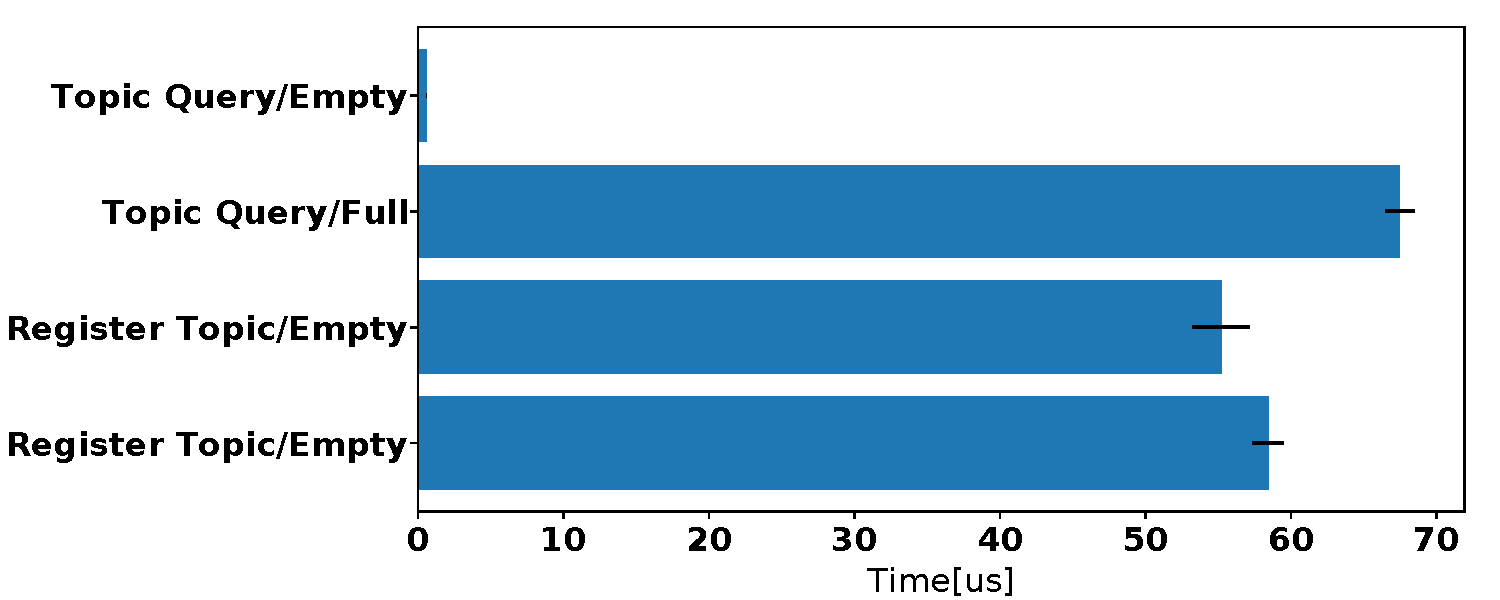
\includegraphics[width=\linewidth]{results/testbed/op_time.pdf}
\caption{Request processing time.}
\label{fig:op_time}
\vspace{-0.15in}
\end{figure}

\subsection{Simulations}

For large scale experiments and comparison with other protocols, we built a prototype of \sysname in PeerSim~\cite{p2p09-peersim}, a scalable P2P network simulator. % In particular, we first implemented the Ethereum DHT by extending a vanilla Kademlia implementation~\cite{peersim_kademlia} with the required changes discussed in ~\Cref{sec:background:dht}. We then built \sysname on top of the Ethereum DHT implementation.

We implement the following approaches as baselines. \textbf{1) \discv} described in \Cref{sec:background:discv4}. \textbf{2) \altname} is a traditional key/value store implementation using the vanilla Kademlia DHT lookup operations.  In this approach, peers store their ads under desired topics at the 20 closest (by DHT distance metric) nodes to the corresponding topic ID. In \altname, registrars accept all incoming ad registrations right away (\ie with no waiting time) and use a simple Last Recently Used (LRU) as a replacement policy. This solution is currently used in InterPlanetary File System (IPFS)~\cite{} - the largest storage network~\cite{libp2p_kaddht}. \textbf{3) \altnameticket} is an extension of \altname. Unlike \altname, this approach uses \sysname's admission control mechanism (\Cref{sec:waitingTime}) regulating the storage of incoming registrations. 

%Many existing systems including the InterPlanetary File System (IPFS)---a decentralised content storage and sharing system---perform peer discovery using the \altname approach~\cite{libp2p_kaddht}. Therefore, we use \altname as a baseline solution in our experiments. 
%As similarly done in the IPFS system, we use N=20 peers (\ie closest to the desired topic's hash) for storage of ads in both \altname and \altnameticket approaches.

%The topic lookup process in \altname and \altnameticket involve first finding N closest peers to the topic using the key lookup process of the Ethereum DHT (\Cref{sec:background:dht}). Once it terminates with a stable list of closest peers, a searcher locally sorts those peers based on their distance (using Kademlia's XOR metric) to the topic's hash. Finally, the searcher queries $\alpha=3$ peers at a time, proceeding with the farthest to the closest of the N peers.


\para{Metrics} We report the following performance metrics. 
 \begin{itemize}
     \item \textbf{Message Overhead} - the total number of messages received by each node. 
%We calculate separate values for both lookup and registration operations. 
Higher values mean larger strain put on each node. 
     \item \textbf{Discovered Peers} - the number of application-specific peers discovered by the searchers during lookup operations. This metric is a measure of the topic search performance by the peers.
%Each operation is finished after discovering 30 nodes. 
     \item \textbf{Discovered By} - the number of searchers each advertiser was discovered by. This metric allows us to verify whether each peer is being discovered and how the number of discoveries differs across peers.
%     \item \textbf{Registrations} - the number of registration placed by each advertiser and the number of registrations each  registrar accepted. It allows to verify the load on each registrar and analyse the their load distribution.
 \end{itemize}
 %We calculate per-node average for the metrics above and report their standard deviation.  Note that \emph{Discovered Peers} and \emph{Discovered By} metric will have the same average vales, but will vary in standard deviation. The same applies to \emph{Placed Registrations} and \emph{Accepted Registrations}. 
 
\noindent
We verify the impact of the following parameters:
 \begin{itemize}
     \item \textbf{Network Size} - the total number of nodes that participate in the discovery. We set the default value to 25,000, as similar number of live nodes were reported by the official Ethereum crawler~\cite{discv4-dns-lists} (\Cref{fig:ecosystem}). We assign each node an IP address and an ID from the crawled ENS records~\cite{bauer2022ethereum}.% We observe an average network churn of 3\% across daily crawls equal and we use this value in our simulations to simulate nodes joining and leaving. 
     \item \textbf{Topics} - the number of distinct applications. We set the default number of topics to 300, which is similar to the observed value by the Ethereum crawler, and also experiment with values 100 and 600. To obtain the number of peers participating in each topic, we use a Zipf distribution with exponent $1.0$ (obtained empirically by fitting the crawler data in \Cref{fig:ecosystem}). 
     \item \textbf{\%Malicious nodes} - the percentage of attackers targeting the peers in the discovery system related to the total number of nodes participating in the topic. We experiment with values ranging from 20\% to 50\%,  using 33.3\% as default value.% Each malicious node is a different Sybil that receives a distinct ID (\ie hash of its public key) generated following a uniformly random distribution.
     \item \textbf{\#Attackers reusing IPs} - the number of attacker nodes reusing the same IP addresses in the attack. Lower values incur increased cost for the attacker. We set its value between 50 and 1, using 5 for the default value.  In our experiments, we use hypothetical attacker IP addresses that have minimum similarity with the set of real IP addresses used by IP addresses (obtained from the crawled ENS records) in order to obtain an upper-bound on the impact of attacks. %At the time of writing this paper, 99\% of the addresses in the Ethereum network are IPv4, and therefore we use only IPv4 addresses in the simulations.

%Meaning that every 25 malicious nodes will share a single, random IP address in the best case or every malicious node will use a different IP address in the worst case.  
 \end{itemize}


Each simulation takes one hour of simulated time during which each advertiser tries to maintain active (\ie unexpired) registrations and each nodes each perform a single lookup operation uniformly spread across the simulation time.  We set the \emph{registration table} capacity to 500 to align with the requirements from the official Ethereum DHT implementation and lifetime $a$ to 15 min.% \ie every 15 min registration expires in the registrars. 

We set all the DHT-related parameters to the ones currently used by Ethereum DHT.%, \ie there are 17 buckets and up to 16 peers stored in each bucket.
%Following Ethereum Kademlia specification,  each bucket has a replacement list of 10 nodes. 
%Every 100 seconds a random bucket is checked for unresponsive nodes. 
%If there are dead nodes, these are substituted by nodes from the replacement list.  If there are not enough nodes in the replacement list,  a new random lookup is performed to discover mode nodes.
Based on formal analysis (see \Cref{sec:analysis}), we set other \sysname parameters such as the number of registrations placed per bucket $K_\textit{register}= 5$, the occupancy exponent $P_\textit{occ} = 10$, the number of peers to contact per bucket during a topic lookup $K_\textit{lookup}=5$, the maximum number of ads a single registrar returns in a lookup $N_\textit{return}=10$. The total number of requested ads peer lookup (\ie $N_\textit{lookup}$) is we set to 30 based on similar requirements of existing applications using Geth.

%The values of these parameters were selected based on extensive simulations that we skip due to the space limitation but included in our Github repository~\cite{our_repo}. 

%%%%%%%%%%%%%%%%%%%%%%%%%%%%%%%%%%%%%%%%%%%%%%%%%%%%%%%%%%%
%\subsection{Message Overhead}
\subsubsection{Evaluation Results}

In the rest of this section, we use violin plots~\cite{violin-plots} for a compact illustration of both the distribution and the density of data points. We limit the shape of the violins within the range of the observed data and set the widths of each data point in the violin proportional to the count of observations at that data point. 
We display the maximum observed values (in red), if the range of the data points exceed the range of the y axis. 


\begin{figure}[!h]
\centering
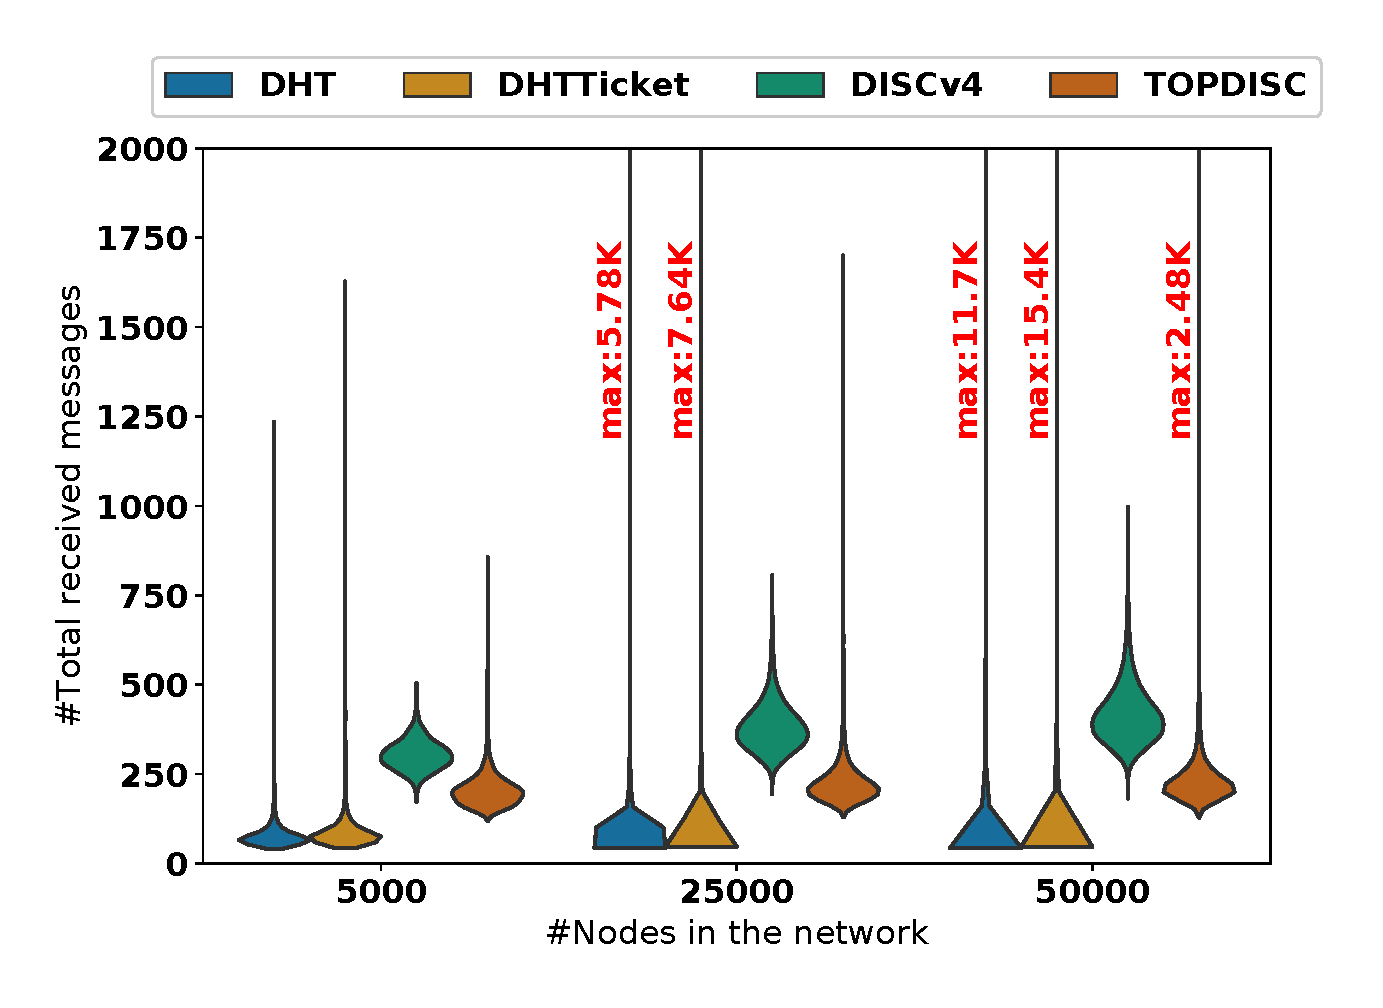
\includegraphics[width=0.470\textwidth]{results/no_split/violin_size_totalMsg.eps}
%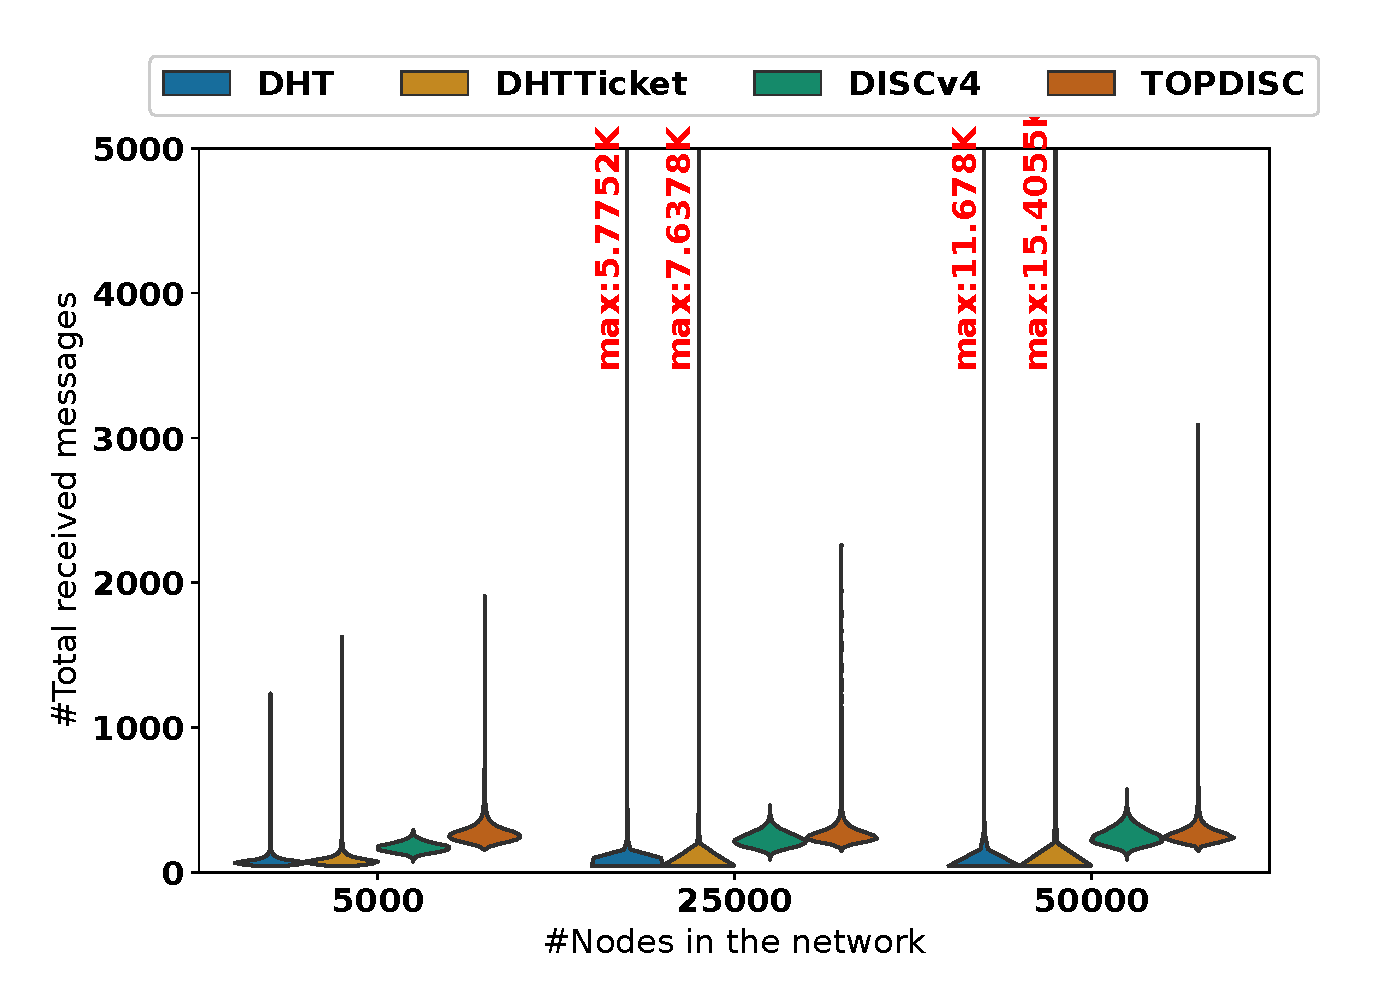
\includegraphics[width=\linewidth]{results/efficiency/violin_size_totalMsg.eps}
\caption{Message overhead for different network size during a single advertisement period.}
\label{fig:msgsPerSize}
\vspace{-0.05in}
\end{figure}

	
\begin{figure}
\centering
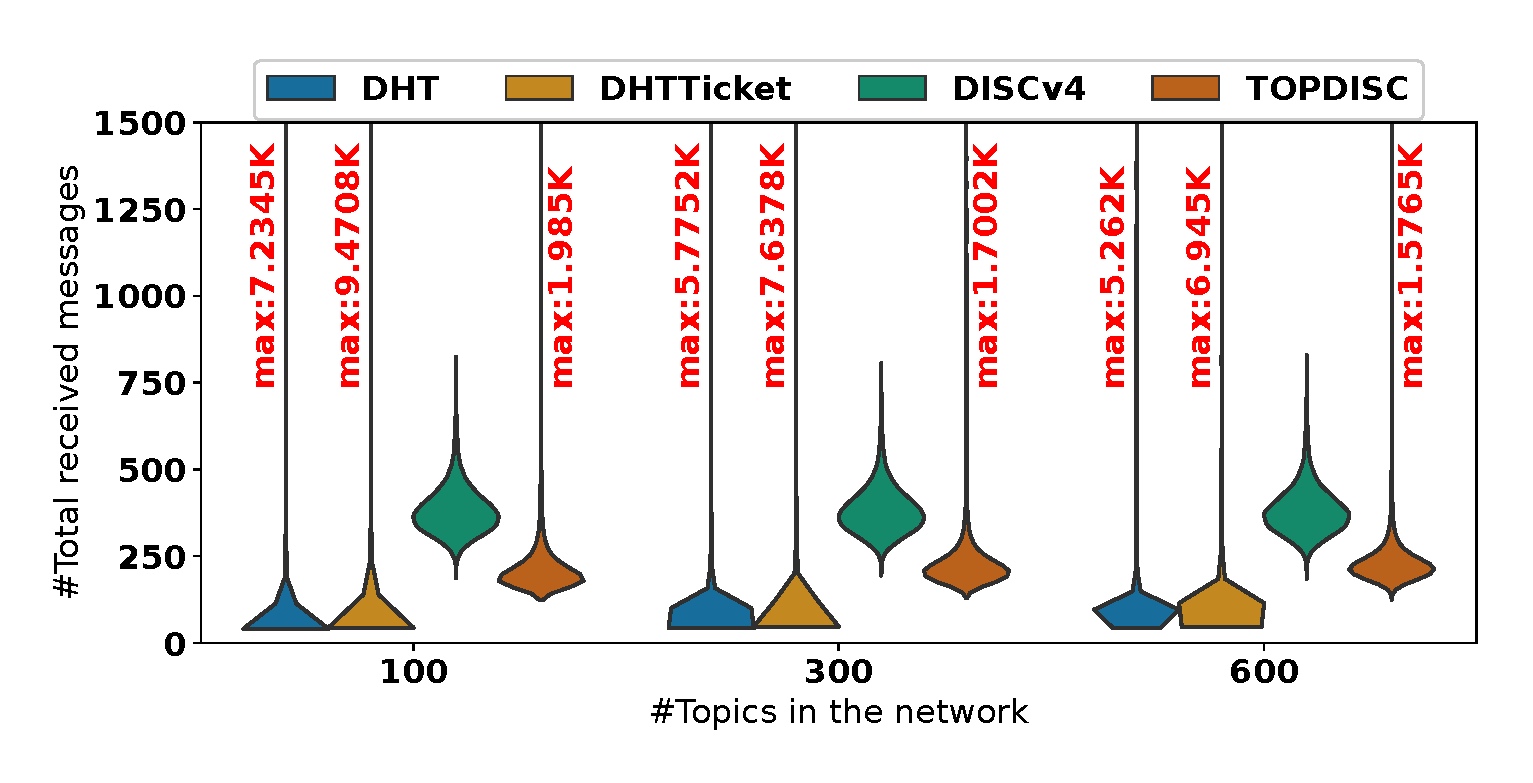
\includegraphics[width=0.470\textwidth]{results/no_split/violin_topic_totalMsg.eps}
%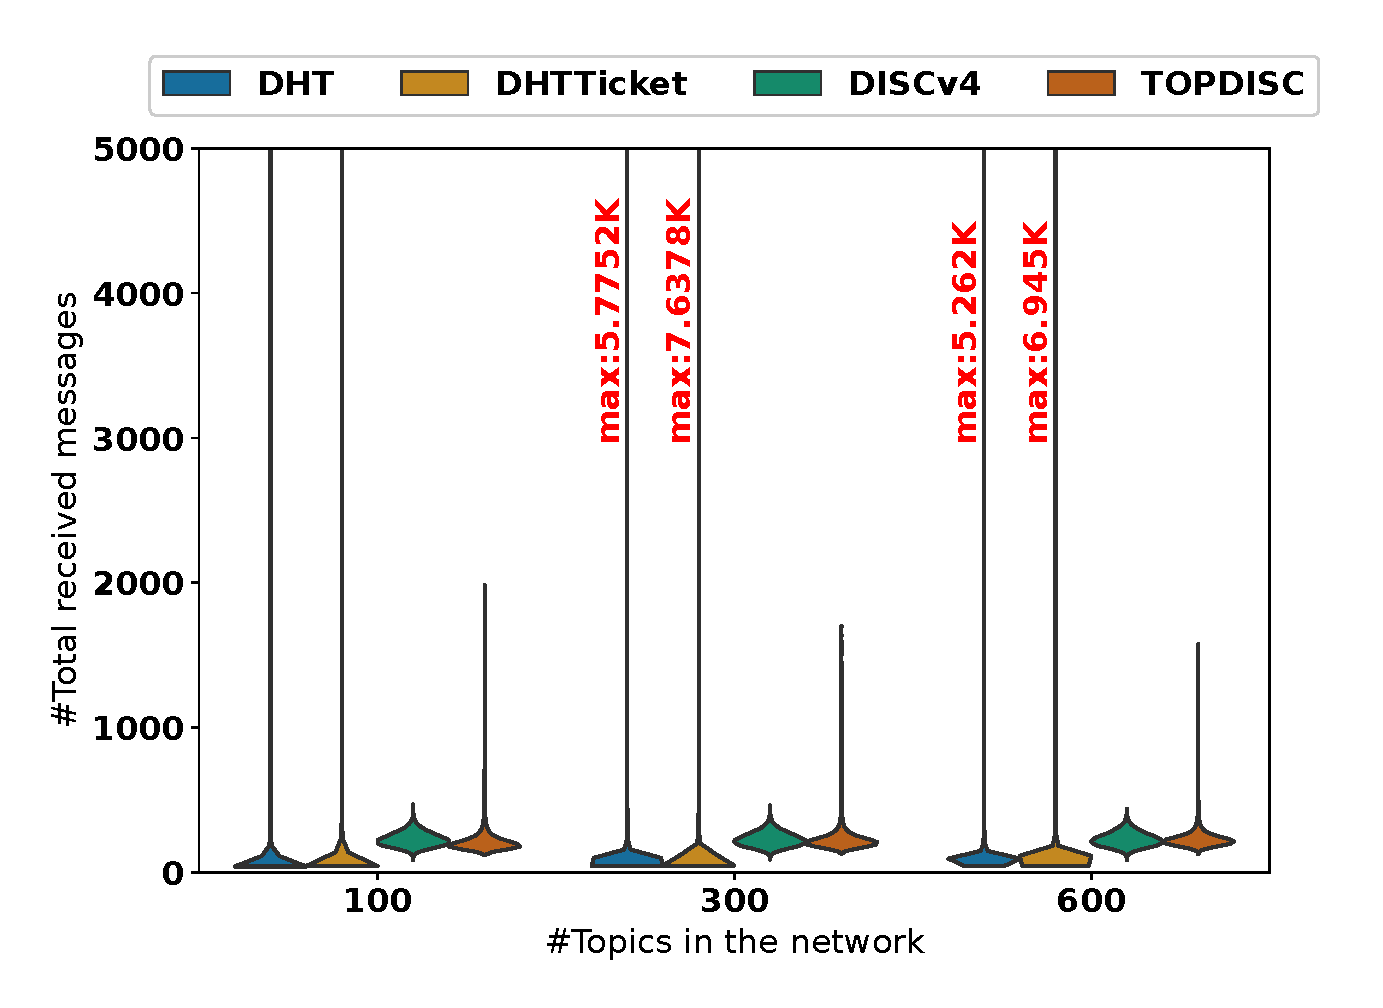
\includegraphics[width=\linewidth]{results/efficiency/violin_topic_totalMsg.eps}
\caption{Message overhead for different number of topics during a single advertisement period.}
\label{fig:msgsPerTopic}
\vspace{-0.15in}
\end{figure}

\para{Network performance}
\Cref{fig:msgsPerSize}~and~\Cref{fig:msgsPerTopic} present \emph{Message Overhead} for the registration and lookup processes. For \discv, only lookups generate messages as there is no registration process in the protocol.
DHT-based protocols introduce low overhead but overload nodes close to popular topic IDs impacting fairness.
The \discv protocol has a better load distribution between nodes since the destination of lookup messages is chosen randomly. However, its message overhead is the highest among all protocols. 
\sysname introduces average overhead but provides more equal load distribution compared to DHT-based protocols.


\begin{figure}[!h]
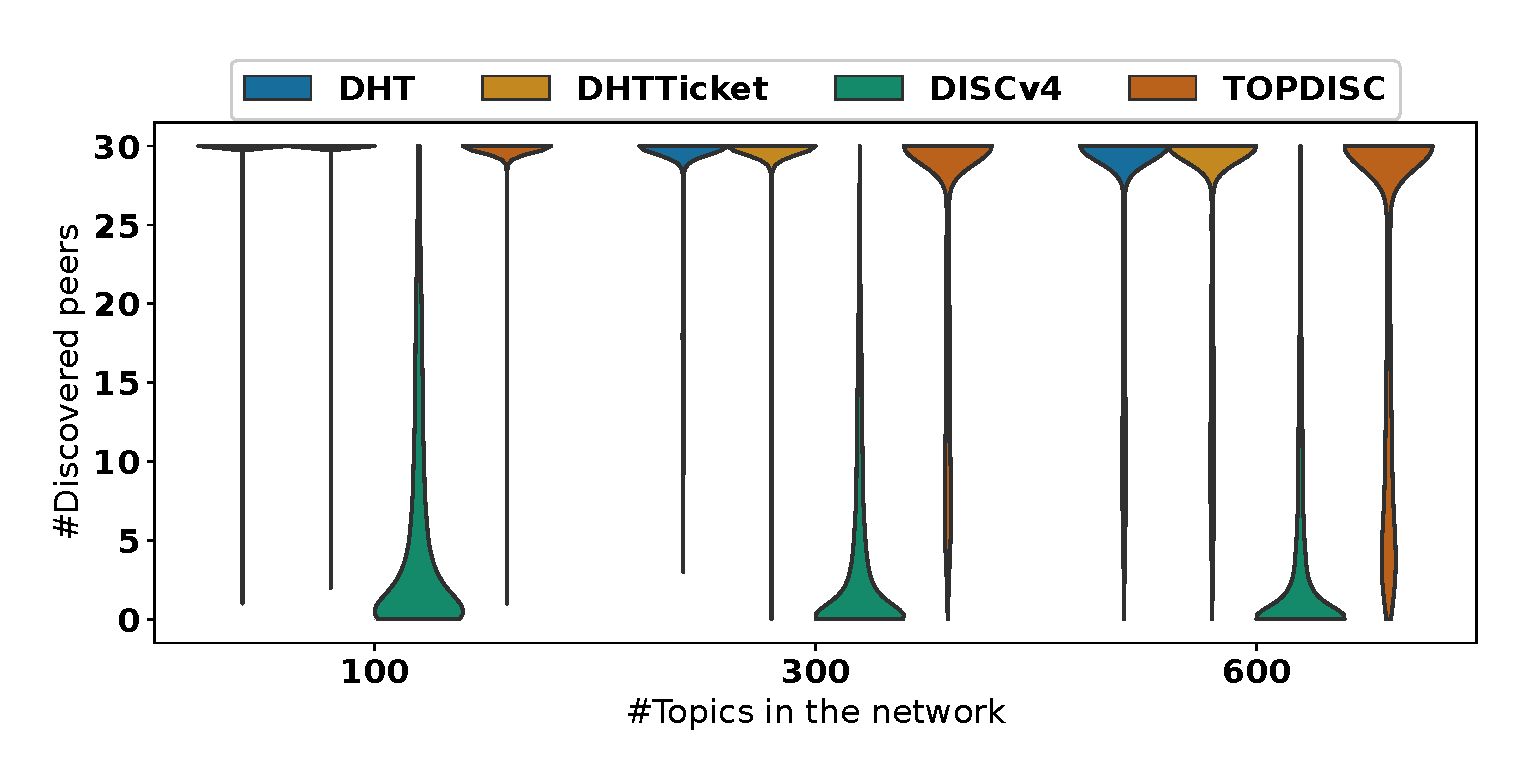
\includegraphics[width=0.470\textwidth]{results/no_split/violin_topic_discovered.eps}
%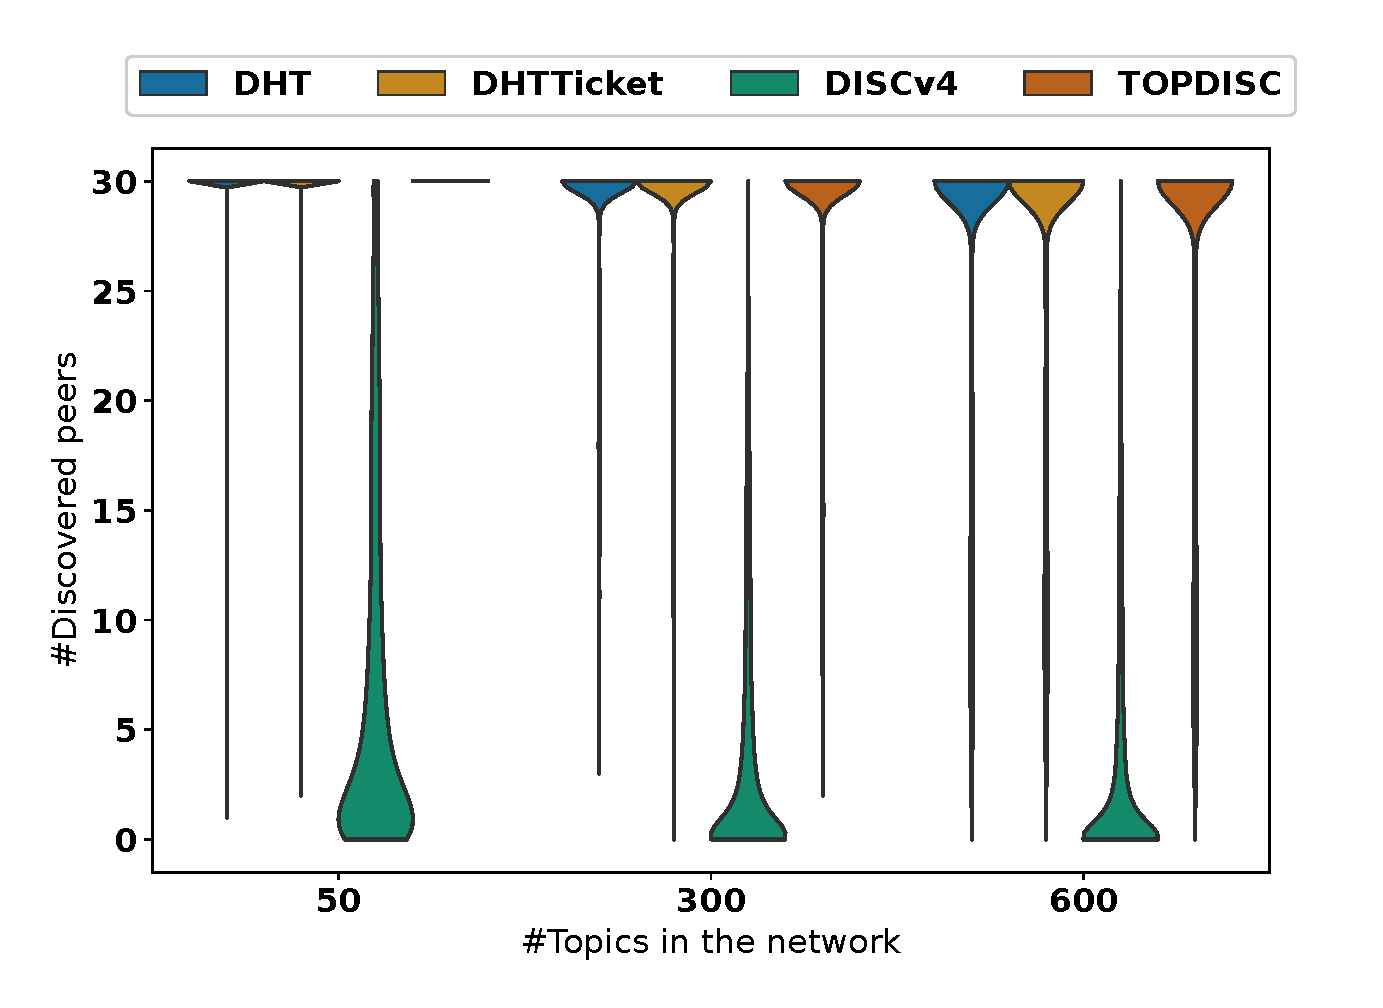
\includegraphics[width=\linewidth]{results/efficiency/violin_topic_discovered.eps}
\vspace{-0.05in}
\caption{Discovered peers for different number of topics.}
\label{fig:discoveredPerTopic}
\end{figure}

\Cref{fig:discoveredPerTopic} presents the number of \emph{Discovered Peers} during a single lookup operation for an increasing number of topics. The random walk of \discv discovers relatively low number of results per operation ($< 5$). The performance decreases with an increasing number of topics in the network. The targeted approach of \sysname and the DHT-based solutions discovers the required number of 30 peers. In rare cases, those protocols do not discover the required amount of peers. It is caused by unpopular topics the total number of participants close to 30. 

%\michal{regarding \Cref{fig:discoveredPerTopic}, it seems that for 300 and 600 topics, we discover slightly less peers on average than the DHT solutions. Why is that? Those results should be for the same topic distributions across protocols, right?}
%\sergi{I think is normal and is caused by the fact that dht is going straight to nodes with most of the registrations so, specially with topics with very few nodes, they can find nodes faster, but with the tradeoff of being eclipsed very easy.}

\begin{figure}[!h]
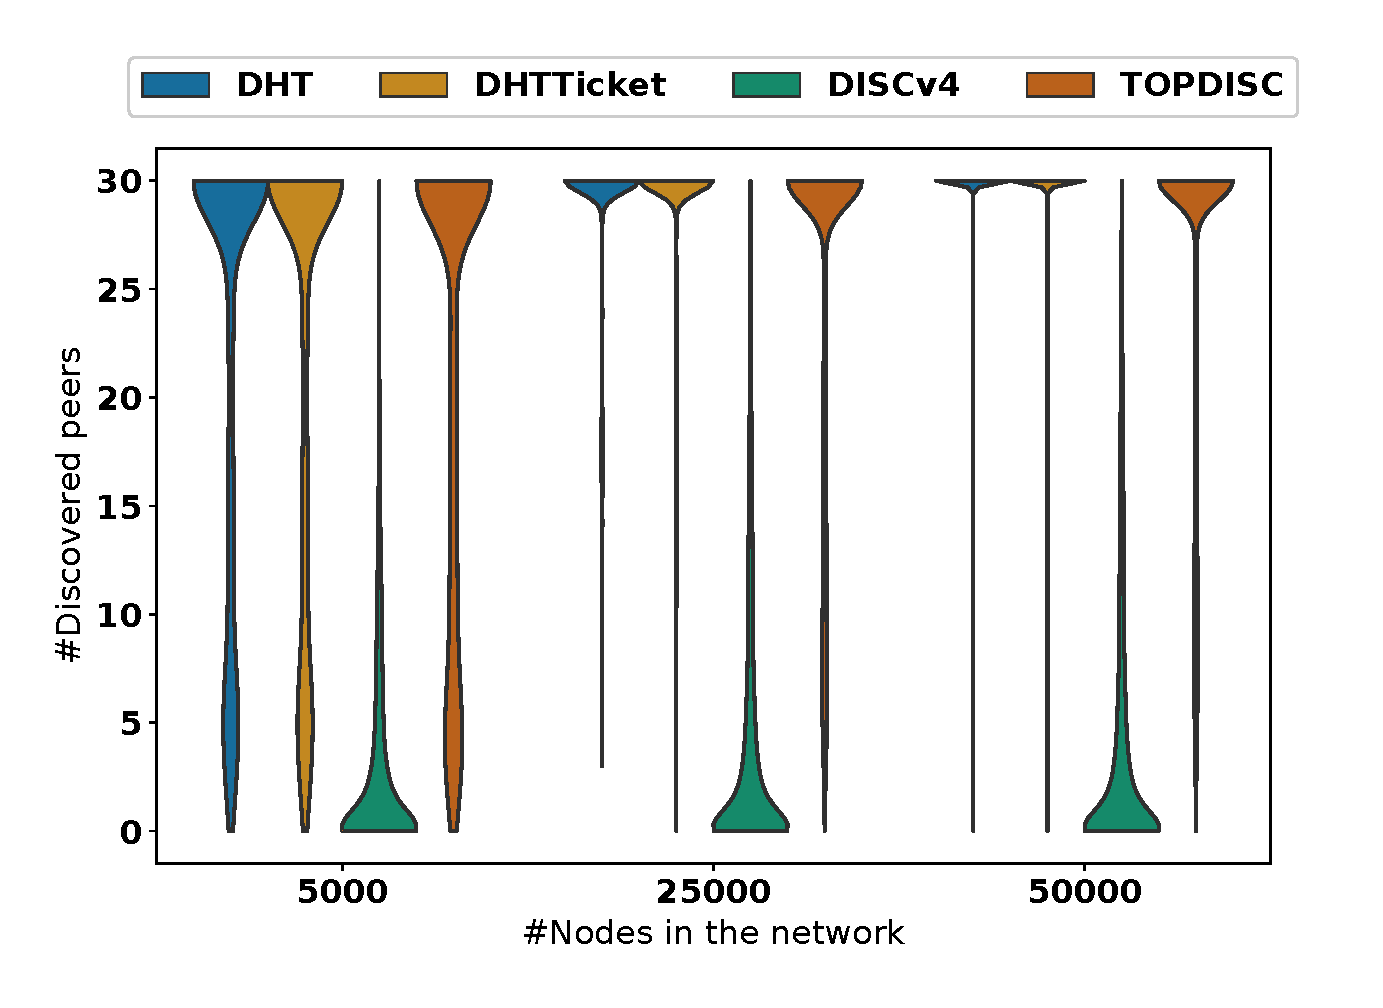
\includegraphics[width=0.470\textwidth]{results/no_split/violin_size_discovered.eps}
%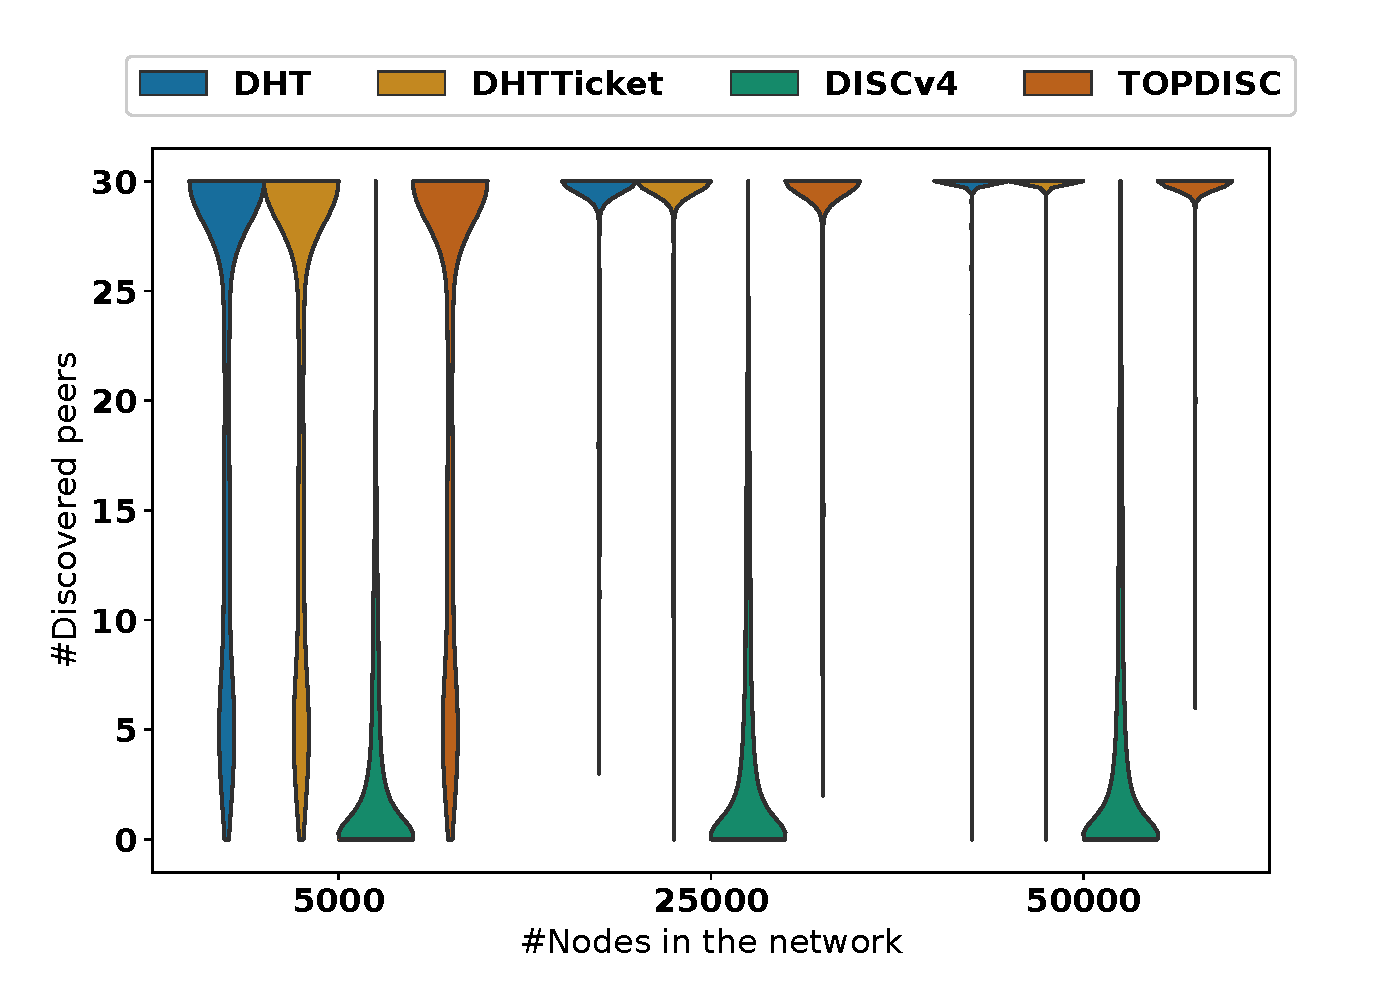
\includegraphics[width=\linewidth]{results/efficiency/violin_size_discovered.eps}
\caption{Discovered peers for different network size.}
\label{fig:discoveredPerSize}
\end{figure}

\Cref{fig:discoveredPerSize} presents \emph{Discovered Peers} during a single lookup operation with an increasing network size. With a fixed number of topics, each application-specific network grows and it is easier to find the required amount of nodes. However, \discv again suffers from poor performance for all the investigated network sizes due to its random movement in the network. 

\iffalse %Onur: removing these for now
\begin{figure}
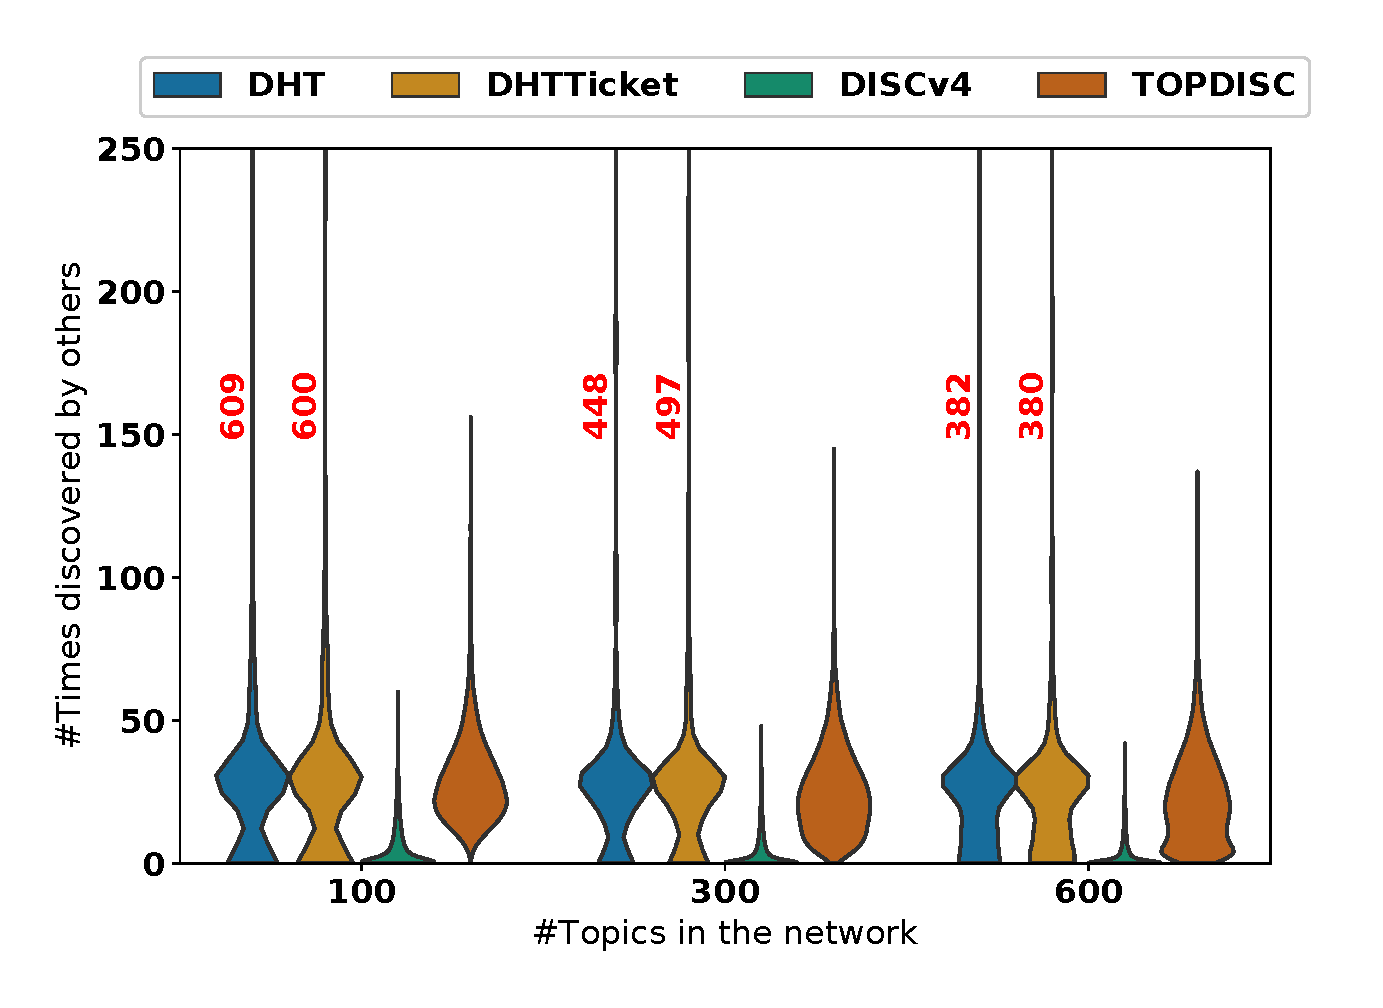
\includegraphics[width=0.470\textwidth]{results/no_split/violin_topic_wasDiscovered.eps}
%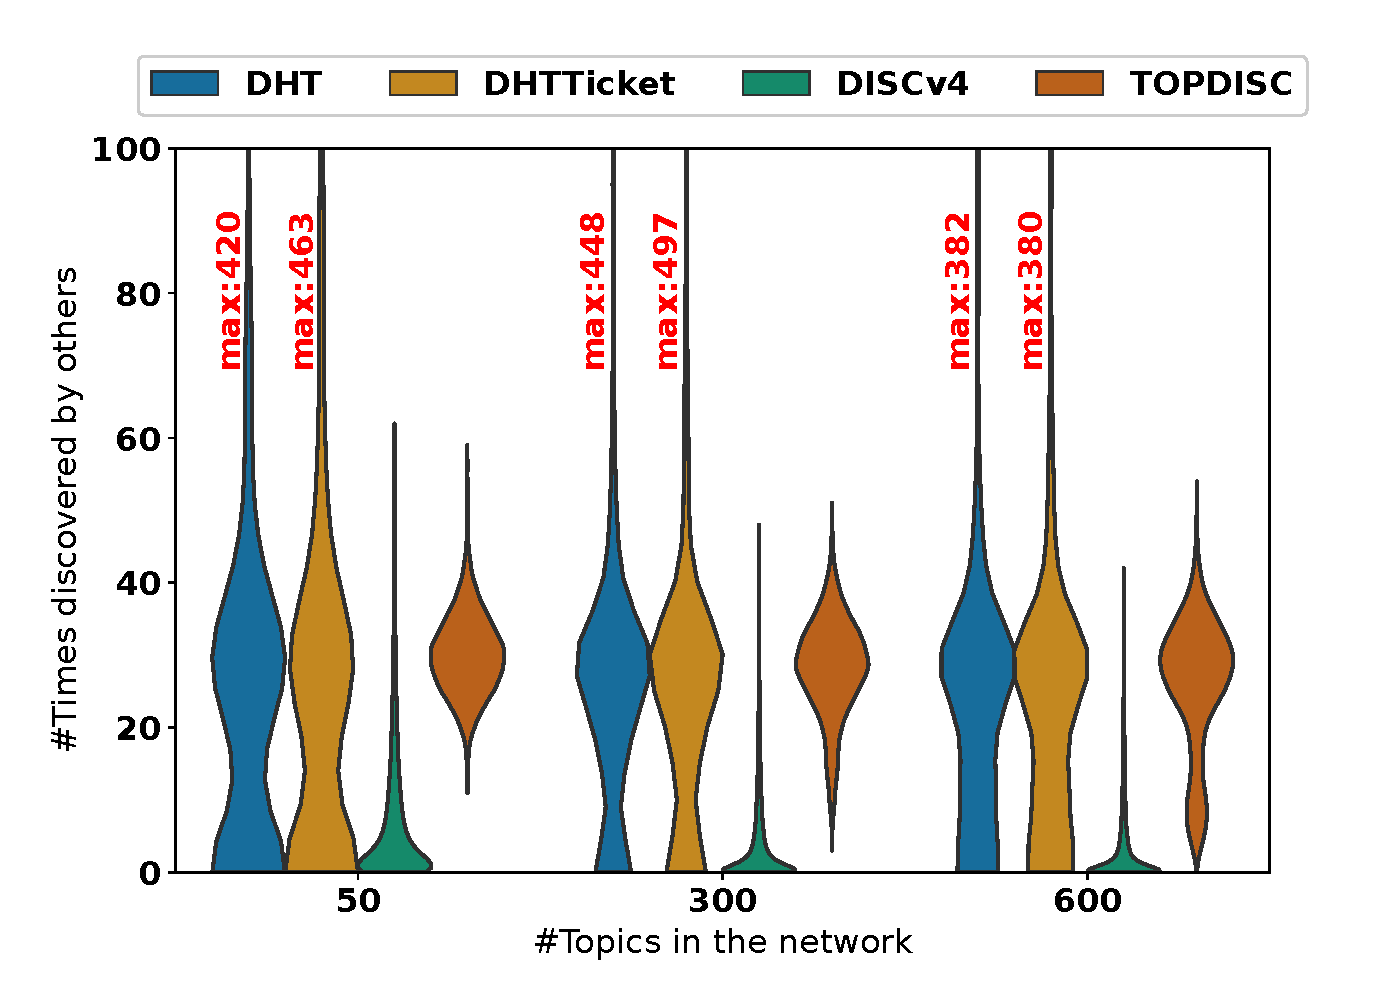
\includegraphics[width=\linewidth]{results/efficiency/violin_topic_wasDiscovered.eps}
\caption{Y-axis: Distribution of the number of times a peer is discovered by others for number of topics in the network for the simulation time.}
\label{fig:discoveredByPerTopic}
\end{figure}

\begin{figure}[!h]
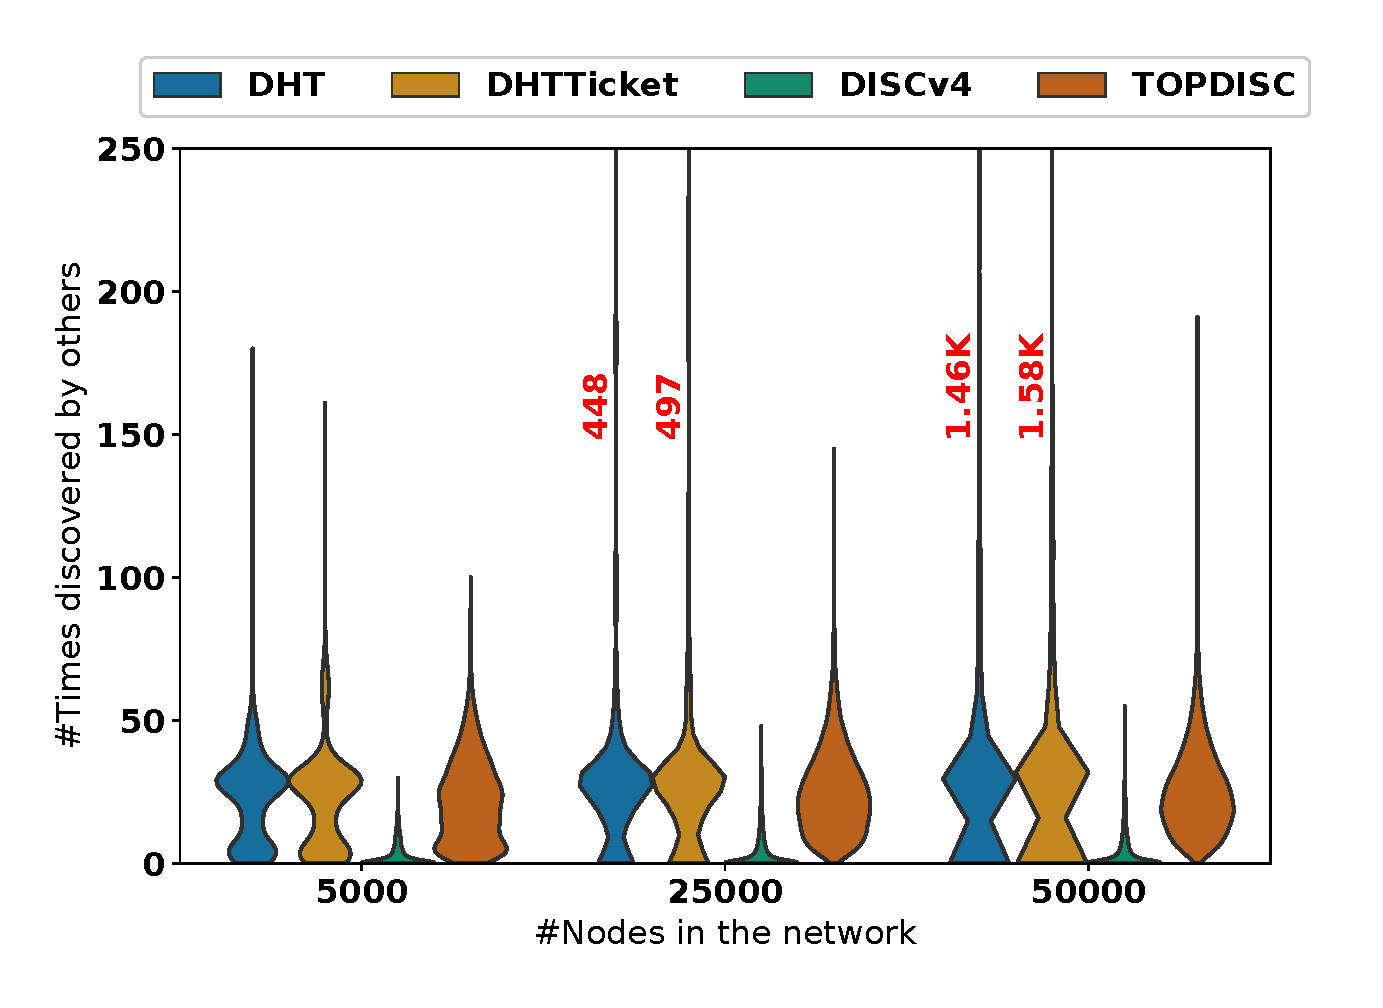
\includegraphics[width=0.470\textwidth]{results/no_split/violin_size_wasDiscovered.eps}
%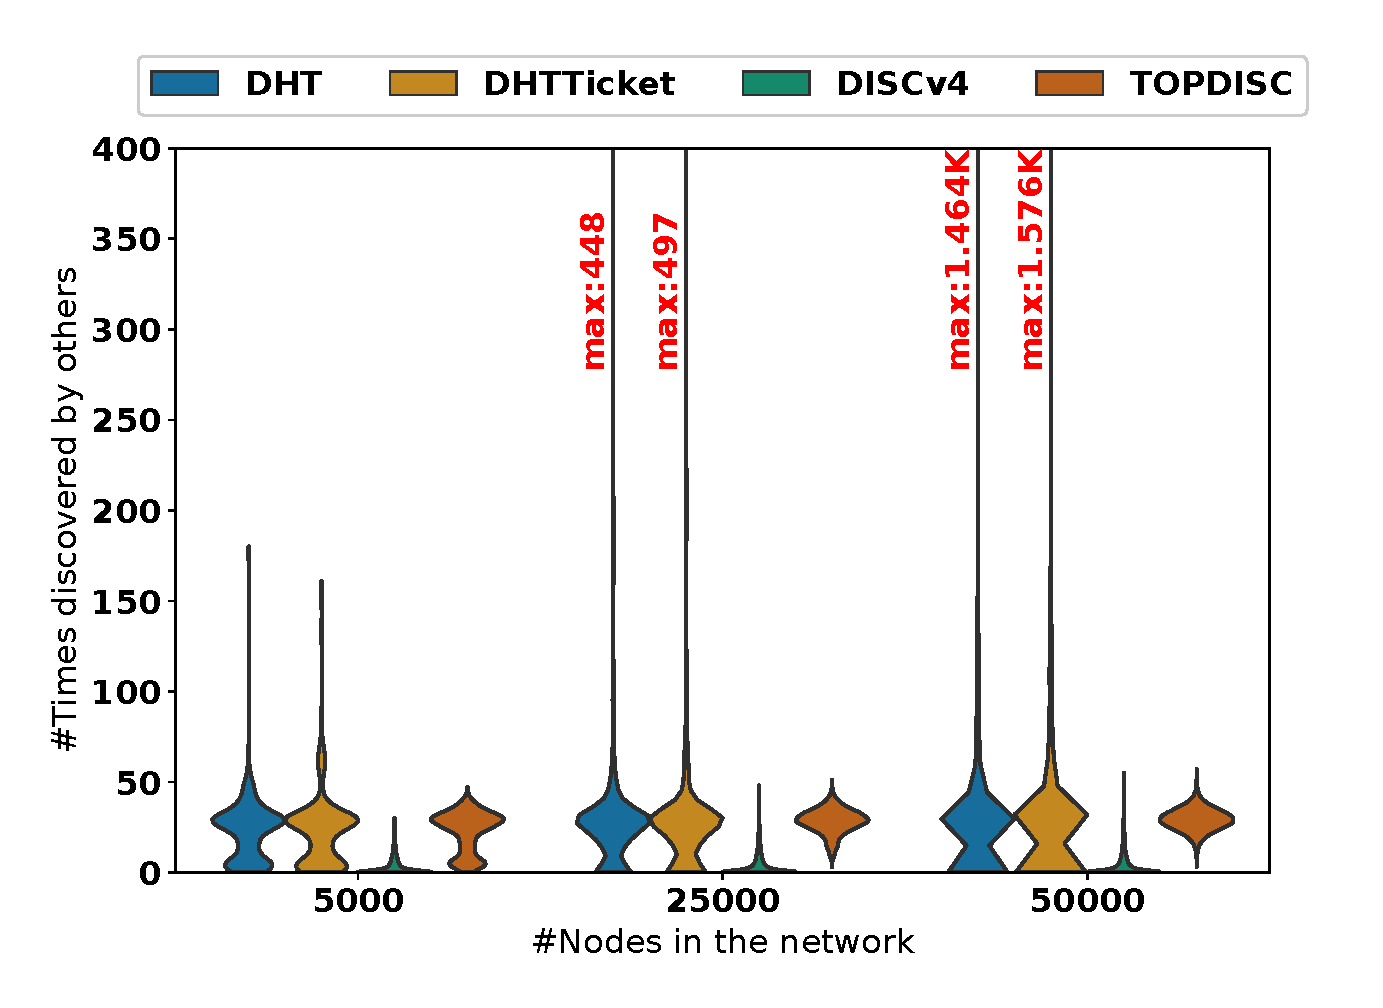
\includegraphics[width=\linewidth]{results/efficiency/violin_size_wasDiscovered.eps}
\caption{Y-axis: Distribution of the number of times a peer is discovered by others for different network size for the simulation time.}
\label{fig:efficiency_size}
\end{figure}
\fi 


\para{Eclipse attack resistance}
We evaluate \sysname resistance against eclipse attacks where an attacker simultaneously behaves as a malicious DHT peer, a malicious registrar and a spamming advertiser (see \Cref{sec:threat}). We consider a lookup eclipse when peers obtained are malicious. We assume a single entity controlling with limited pool of IP addresses coordinating all the malicious nodes. 
Malicious nodes register ads for the targeted topic at a rate 10 times higher than that of honest nodes. Malicious nodes return other malicious peers in response to both DHT routing and topic queries. 

%The objective of the attackers is to eclipse as many peers as possible by taking over their (outbound) connections.
%\discv malicious nodes do not do any registrations and just act as a malicious DHT peer.

%The simulations run for one hour and we report results from a single lookup operation per node for the topic it participates to. 
On top of each violin plot, we specify the \emph{percentage of eclipsed (benign) nodes after a lookup operation}. We assume that the attacker identifiers are uniformly distributed in the address space. We omit the results for scenarios with non-uniform Sybil ID distributions. In that case, the \altname and \altnameticket suffer from $100\%$ eclipse rates. when the attacker places 20 malicious nodes close to a target topic. At the same time, \sysname is shown to achieve lower eclipse rates under a non-uniform Sybil ID distribution (~\Cref{sec:analysis}). The results below represent the worst-case scenario for \sysname and the best-case scenario for protocols we compare against. 
We evaluate the eclipse attacks targeting an average popular topic (approx.  500 nodes participating in the topic). 
%We evaluated the attacks for the most popular and least popular 


%\begin{figure}[!h]
%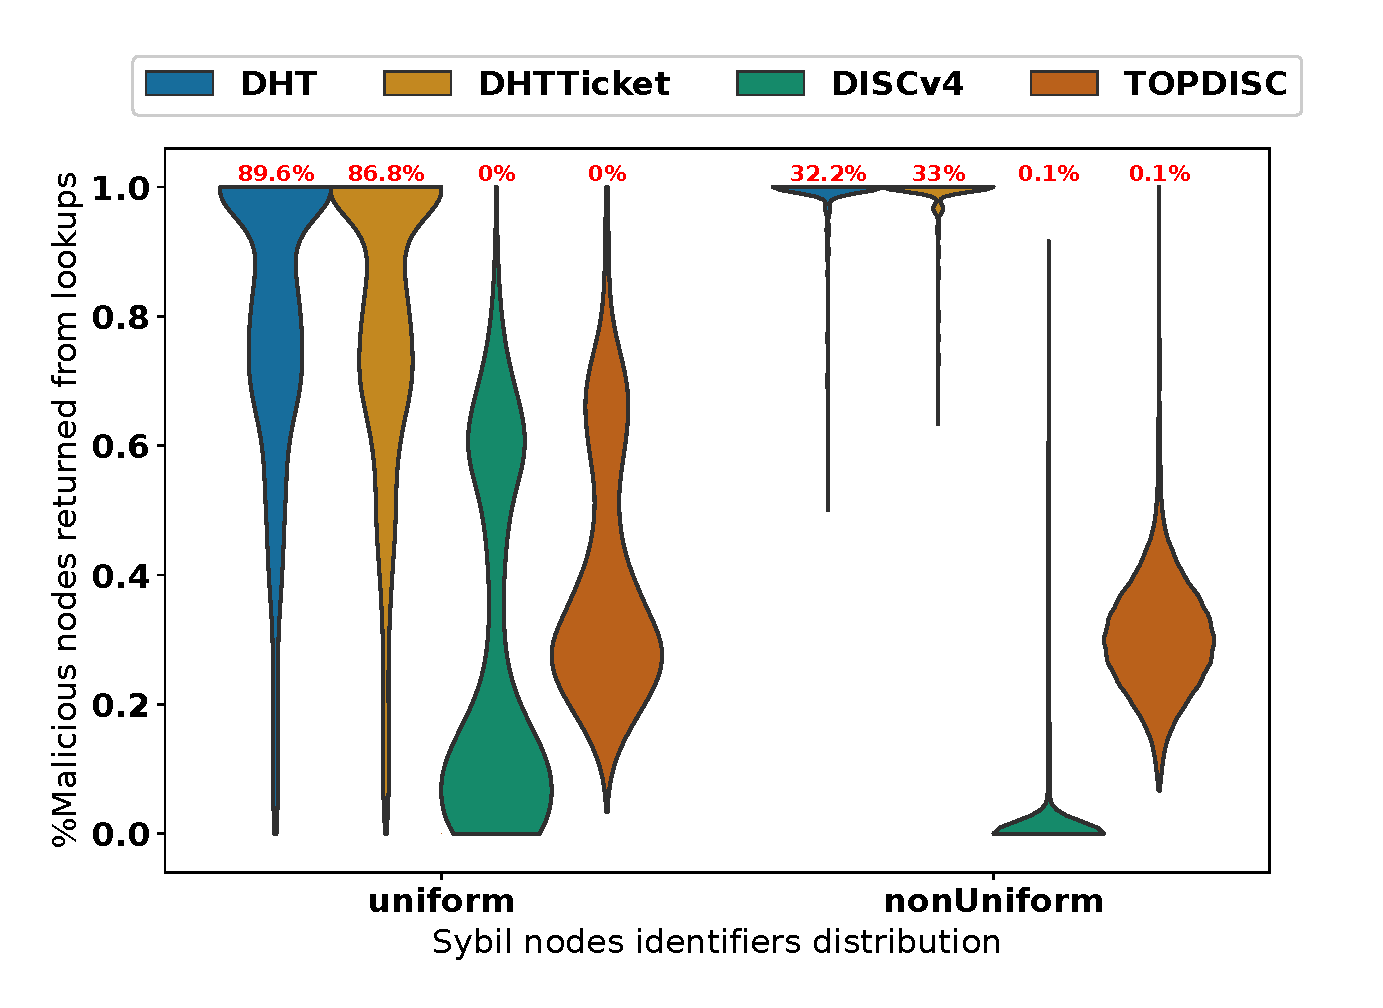
\includegraphics[width=\linewidth]{results/security/violin_idDistribution_percentageMaliciousDiscovered_t0.eps}
%\caption{Y-axis: Malicious nodes discovered and percentage eclipsed nodes using uniform distributed sybil identities vs generating node ids close to topic id,   when attacking the most popular topic (3978 nodes).}
%\label{fig:eclipse_distribution_t0}
%\end{figure}
%
%In Figure~\ref{fig:eclipse_distribution_t0} we show the malicious nodes discovered for all lookups for all protocols using different distribution of the identifiers of the malicious nodes,  when attacking the most popular topic (with 3978 nodes).  In the first option, the malicious nodes ids are artificially generated with a small distance to the topic hash id.  In the second option, malicious nodes identifiers are uniformly distributed.  In the figure we can observe that for \altname and \altnameticket the percentage of eclipses are superior to 80\% because most of the nodes close to topics identifiers are nodes controlled by the attacker.  
%For \altname and \altnameticket, the lookup process is similar to Kademlia lookup process and,  placing all malicious nodes close the topic hash,  it makes very likely to query only malicious nodes during the process, since it only queries the closest known nodes to the topic identifier.
%When attackers are uniformly distributed in the network, eclipses are reduced to close to 32.9\% and 33.7\% respectively.
%Even though it is much less likely to hit malicious nodes during the lookup in this case (remember the default number of malicious are 1000 -4\% of the network-),  when hitting a malicious nodes, the nodes returned by them are used to continue the  query and it may happen it continues querying malicious nodes only during the process.
%When a low popularity topic is attacked (with only 33 nodes),  as shown in Figure~\ref{fig:eclipse_distribution_t299},  for  \altname and \altnameticket the eclipses are even higher, reaching a 100\% of eclipses when placing malicious nodes close to the topic id, and reaching a 78.8\% and 90.9\% when distributing malicious nodes uniformly.  
%Remember the number of attackers is 1000,  against the 33 valid nodes.
%
%For \discv,  the number of eclipses reach is 0\% for the most popular topic when attackers are placed close to the topic hash.  When Sybil nodes are uniformly distributed the number of malicious nodes returned increases,  but to a very low 0.1\%.
%This is caused by the fact that \discv does not target lookups to any specific identifier,  but completely random identifiers,  so it is very difficult for the attackers to place Sybil nodes where they will be queried.  Moreover it is difficult by the attackers to send identifiers where the lookup process will be likely to continue to,  because in the FIND node for the Ethereum DHT the lookup identifier is not disclosed,  but only the distance to it.
%The number of eclipses reach 12.1.\% for the least popular topic when attackers are placed close to the topic hash.  When Sybil nodes are uniformly distributed the number of malicious nodes returned increases,  however the eclipses  reach a 78.8\%.
%The resistance of \discv to Sybil attacks is obtained with the important trade-off of very low efficiency when finding nodes for specific topics, specially for low popular topics.  It is very likely that, when doing lookups using \discv for very low popular topics, no nodes are found or just a few of them.   This means when hitting a malicious node during lookup,  it is likely with a single query to a malicious node, the node querying will be eclipsed.
%
%For \sysname, the number of eclipses are very low for the most popular topic. 
%The eclipses are 0\% when Sybil nodes are placed close to topic id and 0.5\% when are uniformly distributed, with similar distribution to the malicious nodes returned compared with \discv.
%However when attacking the least popular topic the eclipses increase to 78.8\% for both cases.
%This is due to the very low number of valid nodes (33),  that will be more difficult to find than the attackers (1000 nodes, reusing 100 IP addresses).  
%But event the high number of attackers in almost half the cases valid nodes are also found along the evil nodes.
%Remember that Sybil nodes are completely valid nodes from a network discovery point of view when using different network addresses.
%
%\begin{figure}[!h]
%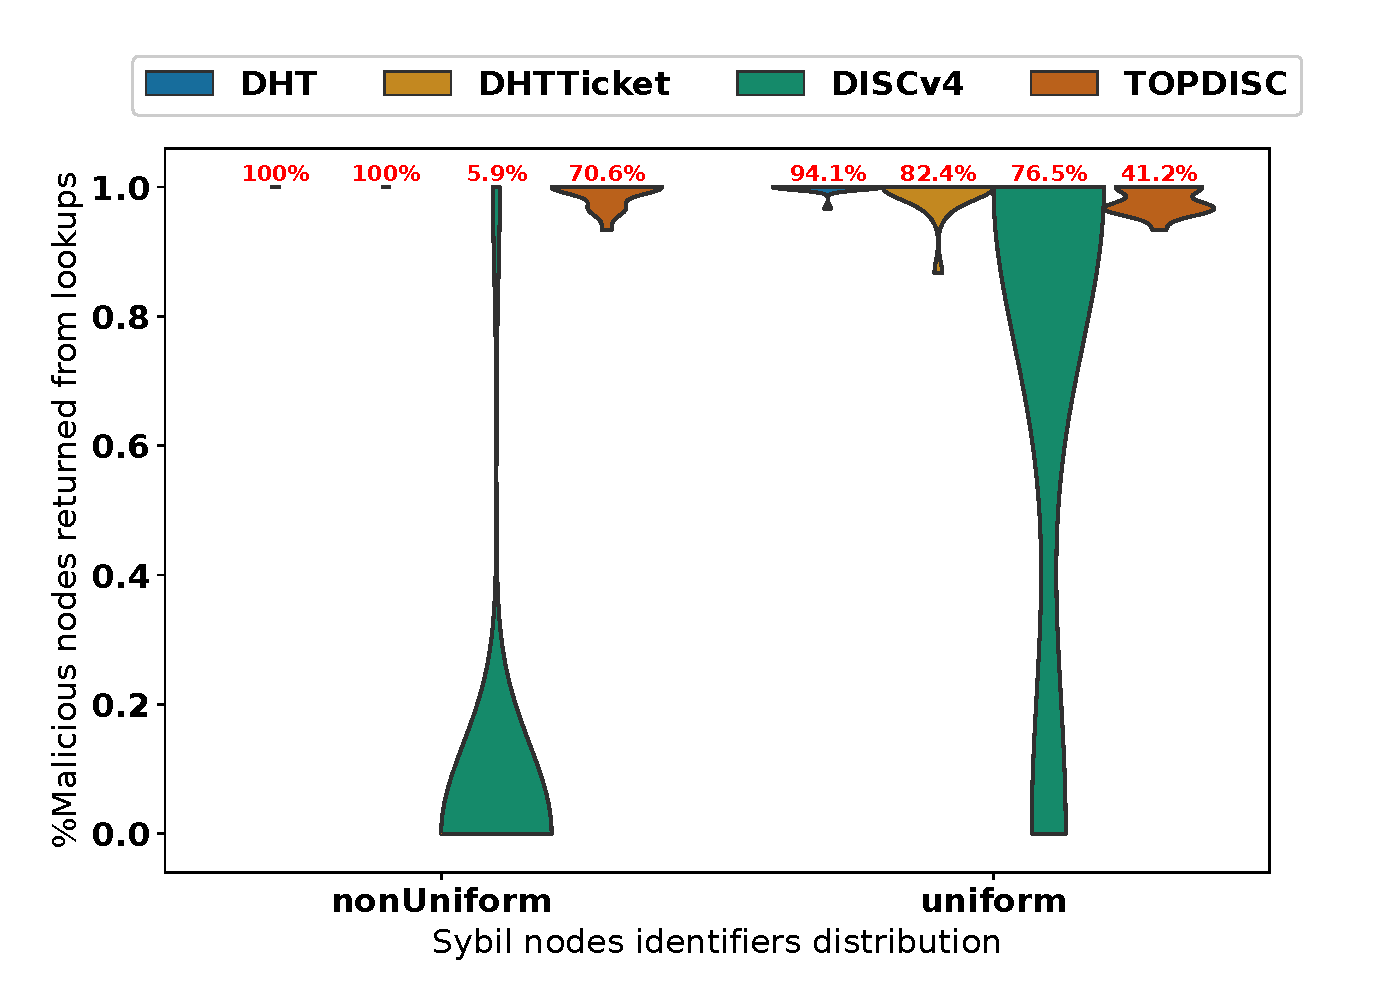
\includegraphics[width=\linewidth]{results/security/violin_idDistribution_percentageMaliciousDiscovered_t299.eps}
%\caption{Y-axis: Malicious nodes discovered and percentage eclipsed nodes using uniform distributed sybil identities vs generating node ids close to topic id,   when attacking the low popularity topic (33 nodes).}
%\label{fig:eclipse_distribution_t299}
%\end{figure}

\Cref{fig:eclipse_evil} presents the percentage of malicious nodes discovered during a single lookup.
The number of malicious node is expressed as a percentage of the total number of system participants. 
% In both figures, Sybil nodes use a pool of 100 IP addresses, and we observe the impact of Sybil size on the eclipse resistance of all four mechanisms. 
\sysname achieves close to a $0\%$ eclipse rate, even with a high number of malicious nodes and is the most resistant protocol.
The admission control mechanism combined with the ad placement strategy form an efficient protection even against attacker controlling $50\%$ of the nodes.
%It highlights the effectiveness of both the waiting time mechanism and distributing the lookup and registration operations across different buckets.
Surprisingly, the random approach of \discv performs worse than \sysname, reaching up to $17.8\%$ eclipse rate. \discv requires querying much more nodes to obtain the required number of peers, and therefore suffers from higher chance of querying malicious nodes.
\altname has  significantly the worse performance, reaching up to 59.7\% eclipse rate.
Thanks to our admission mechanism, \altnameticket outperforms both \discv and \altname resulting in up to $6.5\%$ eclipse rate.
 
% \vspace{-0.20in}
%
%\begin{figure}[!h]
%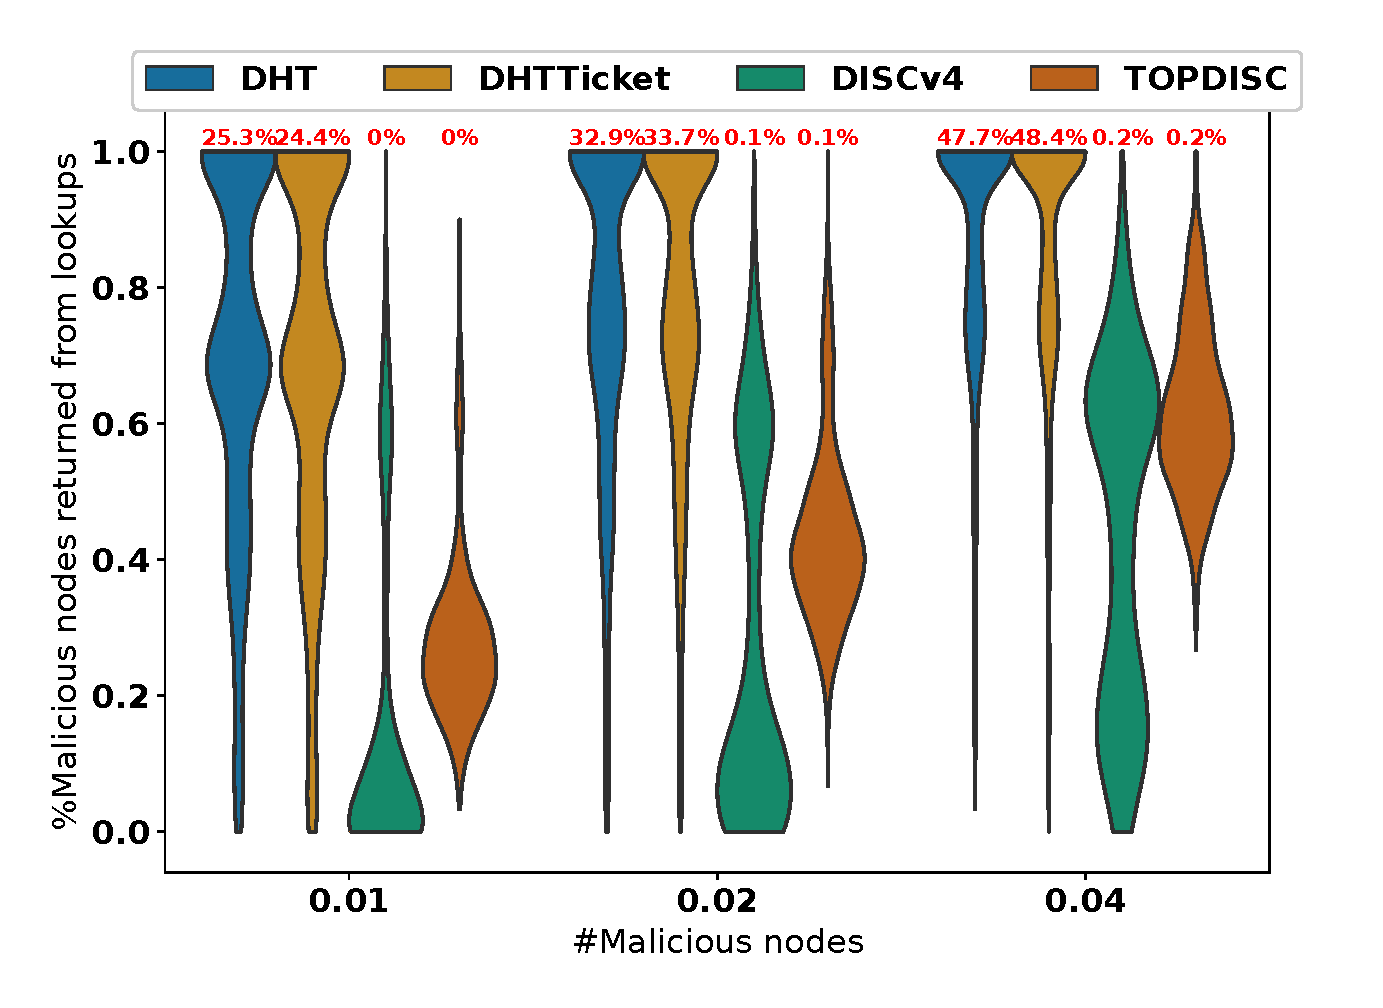
\includegraphics[width=\linewidth]{results/security/violin_percentEvil_percentageMaliciousDiscovered_t0.eps}
%\caption{Y-axis: Malicious nodes discovered and percentage eclipsed nodes for a different number of Sybil nodes used in the attack when attacking the most popular topic (3978 nodes).}
%\label{fig:eclipse_evil_t0}
%\end{figure}

\begin{figure}[!h]
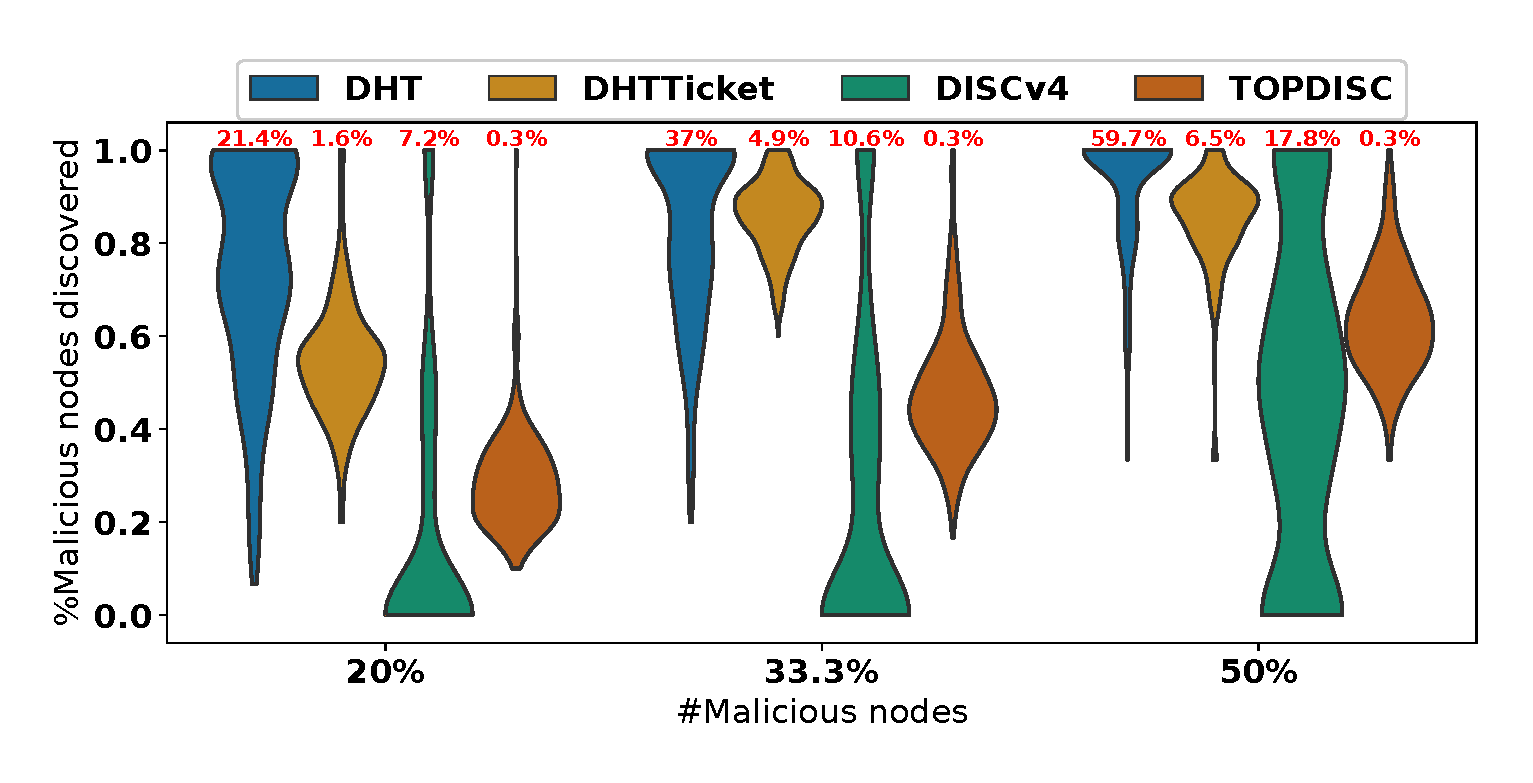
\includegraphics[width=\linewidth]{results/security/violin_percentEvil_percentageMaliciousDiscovered_t10.eps}
\caption{Lookup eclipse rate for a different number of Sybil nodes used in the attack.}
\label{fig:eclipse_evil}
\end{figure}

\Cref{fig:eclipse_sybil} illustrates the percentage of malicious nodes in the lookup results and the lookup eclipse rate. We vary the size of the IP address pool used by the adversary. Value $1$ means that each malicious node has a unique IP address (resulting in high monetary cost for the attacker). An increasing number of IPs used by the attacker makes \sysname more likely to get eclipsed as the the attacker IP score in the waiting function will be similar values received by honest nodes.
Even for the worst case scenario, \sysname achieves the eclipse rate close to $0\%$ to $0.5\%$.
%In comparison, \discv, \altname and \altnameticket are outperformed by \sysname.
%\altname has the worst performance,  followed by \discv with no affectation by the increase of number of IPs used,  since it has no protection agains reusing IP addresses in the attack.
\altname and \discv suffer from significantly higher but remain unaffected by the increasing number of the IP addresses used. Including the admission protocol, allows \altnameticket to outperform the other baseline protocol. However, the regular, DHT-based placement policy is more susceptible to eclipsing compared to \sysname.

%\discv and \altname, with a number of eclipses from $2.8\%$ to $11.4\%$. 
%The number of eclipses are increased for \altnameticket when increasing the number of IPs used in the attack,  since the waiting time admission mechanism limits the number of Sybils accepted in the registration when reusing IPs.

\begin{figure}[!h]
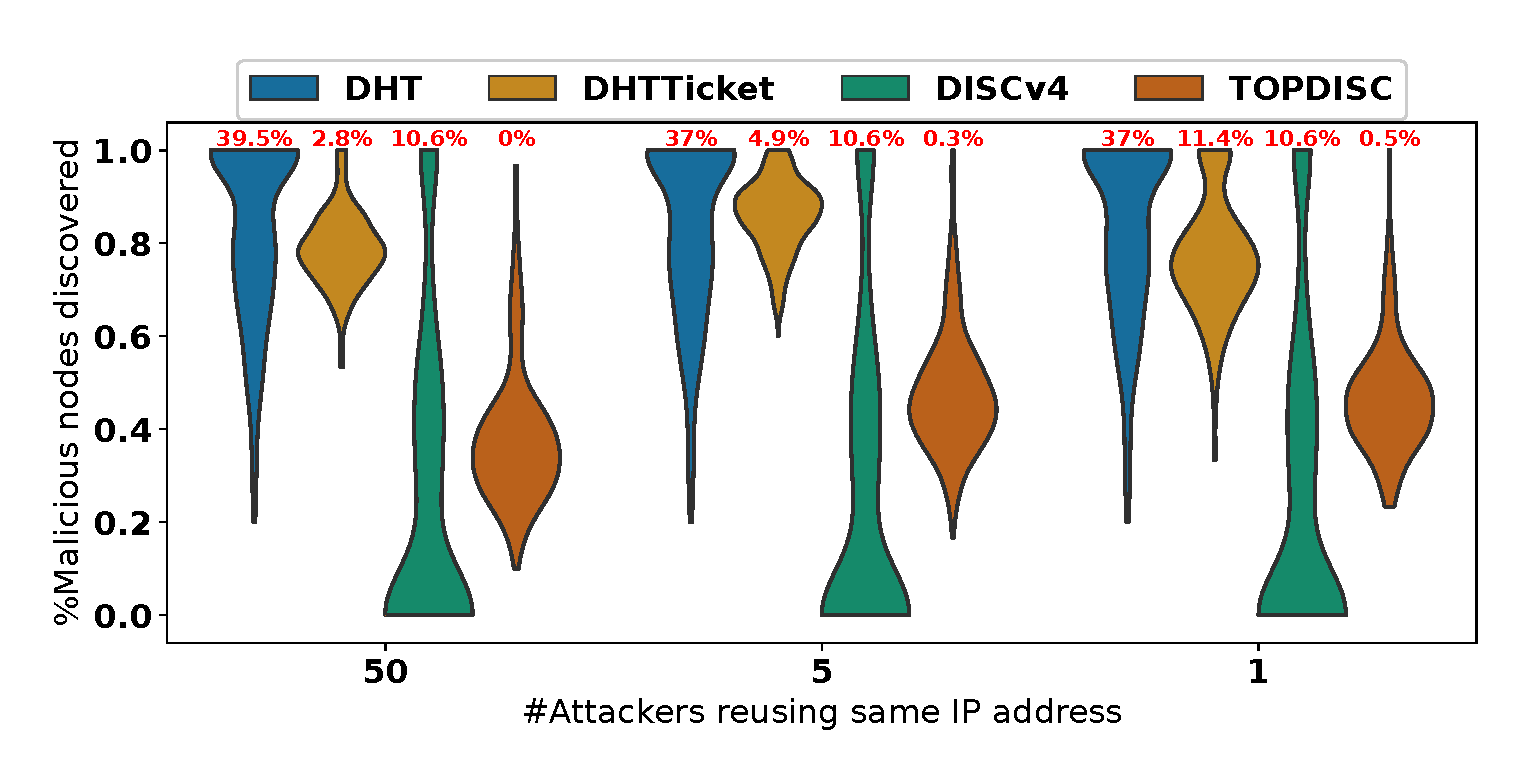
\includegraphics[width=\linewidth]{results/security/violin_sybilSize_percentageMaliciousDiscovered_t10.eps}
\caption{Lookup eclipse rate for a different number of IP addresses used by Sybil nodes.}
\label{fig:eclipse_sybil}
\end{figure}

%\vspace{-0.20in}
%
%\begin{figure}[!h]
%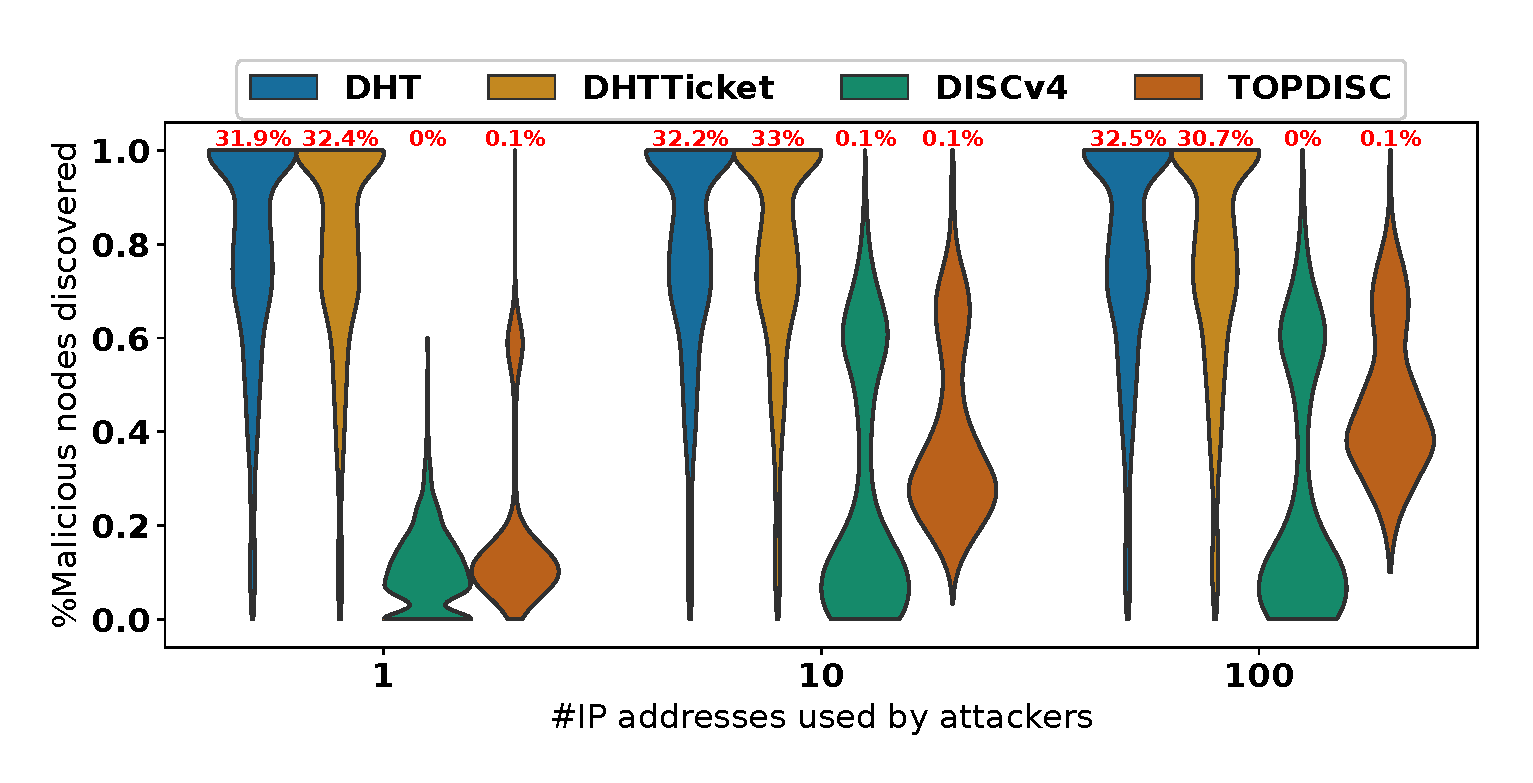
\includegraphics[width=\linewidth]{results/security/violin_sybilSize_percentageMaliciousDiscovered_t0.eps}
%\caption{Y-axis: Malicious nodes discovered and percentage eclipsed nodes for different numbers of IP addresses used in the attack when attacking the most popular topic (3978 nodes).}
%\label{fig:eclipse_sybil_t0}
%\end{figure}
%
%
%\begin{figure}[!h]
%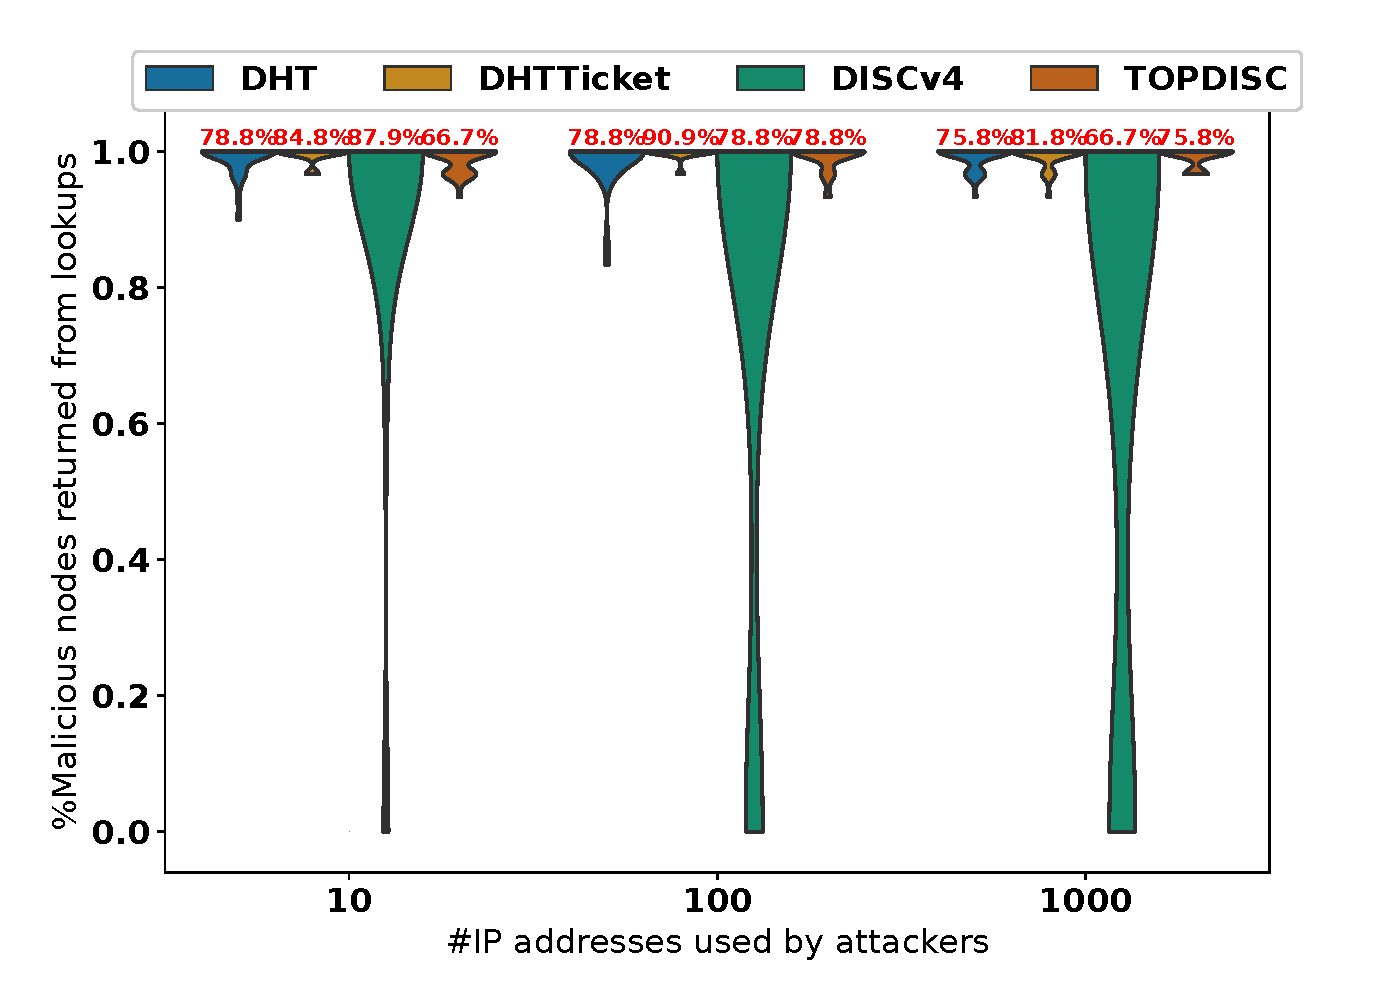
\includegraphics[width=\linewidth]{results/security/violin_sybilSize_percentageMaliciousDiscovered_t299.eps}
%\caption{Y-axis: Malicious nodes discovered and percentage eclipsed nodes for different numbers of IP addresses used in the attack when attacking the least popular topic (33 nodes).}
%\label{fig:eclipse_sybil_t299}
%\end{figure}








%\begin{figure*}[!h]
%\centering
%\subfigure[{Y-axis: Percentage eclipsed nodes using uniform distributed sybil identities vs generating node ids close to topic id}]{
%\includegraphics[width=0.31\textwidth]{results/security/%bar_idDistribution_percentageEclipsedLookups_t0.eps}
%violin_idDistribution_percentageMaliciousDiscovered_t0.eps}
%\label{fig:distribution}
%}
%\subfigure[{Y-axis: Percentage eclipsed nodes for different number of sybil nodes in the attack.}]{
%\includegraphics[width=0.31\linewidth]{results/security/%bar_percentEvil_percentageEclipsedLookups_t0.eps}
%violin_percentEvil_percentageMaliciousDiscovered_t0.eps}
%\label{fig:percentEvil}
%}
%\subfigure[{Y-axis: Percentage eclipsed nodes for different number IP addresses used in the attack.}]{
%\includegraphics[width=0.31\linewidth]{results/security/%bar_sybilSize_percentageEclipsedLookups_t0.eps}
%violin_sybilSize_percentageMaliciousDiscovered_t0.eps}
%\label{fig:sybilsize}
%}
%\caption{Resistance against eclipse attacks when attacking most popular topic (t0)} 
%\label{fig:eclipse_attack}
%\vspace{-0.05in}
%\end{figure*}
%
%\begin{figure*}[!h]
%\centering
%\subfigure[{Y-axis: Percentage eclipsed nodes using uniform distributed sybil identities vs generating node ids close to topic id}]{
%\includegraphics[width=0.31\textwidth]{results/security/%bar_idDistribution_percentageEclipsedLookups_t299.eps}
%violin_idDistribution_percentageMaliciousDiscovered_t299.eps}
%\label{fig:distribution}
%}
%\subfigure[{Y-axis: Percentage eclipsed nodes for different number of sybil nodes in the attack.}]{
%\includegraphics[width=0.31\linewidth]{results/security/%bar_percentEvil_percentageEclipsedLookups_t299.eps}
%violin_percentEvil_percentageMaliciousDiscovered_t299.eps}
%\label{fig:percentEvil}
%}
%\subfigure[{Y-axis: Percentage eclipsed nodes for different number IP addresses used in the attack.}]{
%\includegraphics[width=0.31\linewidth]{results/security/%bar_sybilSize_percentageEclipsedLookups_t299.eps}
%violin_sybilSize_percentageMaliciousDiscovered_t299.eps}
%\label{fig:sybilsize}
%}
%\caption{Resistance against eclipse attacks when attacking least popular topic (t299)} 
%\label{fig:eclipse_attack}
%\vspace{-0.05in}
%\end{figure*}
%\begin{figure}[!h]
%\includegraphics[width=\linewidth]{img/placeholder}
%\caption{Compare only against DHT here I guess? Y-axis a ratio of popular malicious and benign ads in the table for spam attack and topic-targeted attack within a single registrar. X-axis: to avoid showing different graphs for multiple malicious IPs/IDs/nodes we can have a fix ratio between them i.e., each 5 Sybils (or requests/s) have 1 IP and 2 ID, and increase this "attacker strength".} 
%\label{fig:security_spam}
%\end{figure}
%
%\begin{figure}[!h]
%\includegraphics[width=\linewidth]{img/placeholder}
%\caption{Compare only against DHT here I guess? Y-axis a  time to discovery/registration (do we care about registration if lookup works?) slowdown compared to a non-attack scenario?Do we consider different placements of Sybils here (i.e., only bucket 1? Or spread evenly across all the buckets?). X-axis: to avoid showing different graphs for multiple malicious IPs/IDs/nodes we can have a fix ratio between them i.e., each 5 Sybils have 1 IP and 2 ID, and increase this "attacker strength".} 
%\label{fig:security_spam}
%\end{figure}



\iffalse
\subsection{Performance Results}
\michal{We should group the result so that they show achievement of specific goals that we described before}

%\paragraph{Ticket registrations:
In the following we detail the performance evaluation in four different subsections.  In the first we show the registration performance.  Secondly we show the traffic load and overhead of the designed mechanism.  Then we continue with the lookup and discovery performance and we finish with the security analysis.

\subsubsection{Registration  performance}

In Figure~\ref{fig:regs} we observe the average active registrations in the system per topic with different number of nodes in the simulation,  from 500 to 10000 nodes. 
We can observe nodes for all topics are able to place a substantial amount of registrations, even the less popular topics. 
As number of nodes increase in the network, we can observe the differences between registrations per topic are reduced. 
Actually, it can be observed the most popular topic (t1) is able to place less registrations than t2. 
This is caused by the fact that with more nodes trying to register for the same topic,  waiting times increase.
If the waiting time increases over the waiting time limit (in the simulations is set to 15 min),  the node cancels the registration and tries with a different nodes.
When cancellations happen it may lead to less active registrations, because it may end up with longer registration processes.
In our simulation we observe less registrations for t1 than t2  because t1 registrations waiting time go over the waiting time limit more often.

In Figure~\ref{fig:time_reg} we observe the average time necessary for a node to place a registration,  from 500 to 10000 nodes in the simulation.
We can observe that average registration time is always below 500 seconds and this is reduced for less popular topics and smaller networks. 
This figure does not include registration times for cancelled registrations.
\sergi{I think we should include failed/uncomplete registrations in the plot}

\begin{figure}[!h]
\centering
\subfigure[{Active registrations}]{
\includegraphics[width=0.225\textwidth]{img/eval/registration_origin.eps}
\label{fig:regs}
} 
\hspace{-0.25cm}
\subfigure[{Time to register}]{
\includegraphics[width=0.225\textwidth]{img/eval/avg_time_register.eps}
\label{fig:time_reg}
}
 \caption{Ticket registrations} 
\label{fig:registrations}
\vspace{-0.15in}
\end{figure}   

%\begin{figure}[h!]
%\centering
%%\epsfig{file=imgs/eval/scen5.pdf, width=0.45\textwidth}
%\includegraphics[width=0.225\textwidth]{img/eval/registration_origin.png}
%\caption{Registrations}
%\label{fig:regs}
%\vspace{-0.15in}
%\end{figure}

%\paragraph{\bf{Network load}:}
\subsubsection{Network load}

In Figure~\ref{fig:messages}~and~\ref{fig:msg_distr} we can observe the traffic load generated in the network.
In Figure~\ref{fig:messages} we observe most of the messages are ticket requests/replies, and the subsequent registration request/replies
after receiving a ticket from a node. 
This is caused by the fact that nodes are constantly registering dynamically. 
In Figure~\ref{fig:msg_distr} the messages received distribution. 
We can observe some nodes receive much more messages.
This is caused by the bucket node distribution, where nodes with identifiers close to topic hash ids receive more initial tickets requests because there are less.
However, we observe while the number of nodes in the network is increased 20 times,  the  maximum number of messages received by some nodes does not increase in the same way,  only being twice the amount when comparing 500 with 10000 nodes,  ans with increases lower than 30\% when number of nodes are doubled.
Moreover,  we can also see the number of messages received does not exceed 10 times the average value of the messages received. 

Therefore, the system is able to scale without danger of overloading some of the nodes of the network.

\begin{figure}[!h]
\centering
\subfigure[{Number of messages}]{
\includegraphics[width=0.225\textwidth]{img/eval/message_quantity.eps} 
\label{fig:messages}
} 
\hspace{-0.25cm}
\subfigure[{Message distribution}]{
\includegraphics[width=0.225\textwidth]{img/eval/messages_received.eps} %\hspace{-1.5em}%
\label{fig:msg_distr}
}
 \caption{Traffic load} 
\label{fig:traffic}
\vspace{-0.15in}
\end{figure}   

\subsubsection{Discovery and lookup performance}

%\paragraph{\bf{Discovery performance}:}

In Figure~\ref{fig:reg_disc} and \ref{fig:timedisc} we can observe how nodes are discovered within the network.
In Figure~\ref{fig:reg_disc} we observe the percentage of the nodes in the network that are discovered and how often are discovered.
Each node in the network is represented by a circle, and the size of the circle represents the relative frequency of discoveries compared with other nodes in the network.
We can observe that for all topics the percentage of nodes discovered in the network is very close to 100\%. This means almost all nodes in the network are able to be discovered by other nodes. The number of discovered nodes is not 100\% because of the existence of turbulence (there are some nodes just joined the network and there has not been enough time yet to be discovered). In case there are a low number of nodes for a specific topic (e.g. t5 with 500 nodes network) the 100\% is reached.
We can also observe Figure~\ref{fig:reg_disc} that the discovery distribution is bounded to \hl{X} times between the most discovered and the least discovered.
We observe the dots size are very regular and despite being not completely equal the differences are not substantial. 
In Figure~\ref{fig:timedisc} we observe the time between a registration is completed and the first time the registration
is returned in a lookup.
By observing this we can see how difficult is for a node to be discovered once is able to place a registration. 
We see the average time is between 20 and 10 seconds in most of the cases, except for the least popular topic t5 which is around 50\% higher. 
We also observe the deviation is bounded at around 60 seconds, with equivalent different for t5.


\begin{figure}[!h]
\centering
\subfigure[{Advertiser discovery distribution}]{
\includegraphics[width=0.225\textwidth]{img/eval/registrant_distribution.eps} 
\label{fig:reg_disc}
} 
\hspace{-0.25cm}
\subfigure[{Time between registration and first discovery}]{
\includegraphics[width=0.225\textwidth]{img/eval/min_time_discovery.eps} %\hspace{-1.5em}%
\label{fig:timedisc}
}
 \caption{Discovery performance} 
\label{fig:discovery}
\vspace{-0.15in}
\end{figure}   


In Figure~\ref{fig:hopcount} we can observe the lookup performance of \sysname compared with \discv for a 5000 nodes simulation.
In the plot we show the average number of nodes discovered for each hop during a lookup per topic, taking into account that \discv cannot do per topic lookups,  so we discard received nodes that do not support the specific service.
In the figure we observe that for t1 the discovered nodes are higher when using \discv, since all topics support t1 and any node discovered will be a valid node. 
However, as the popularity of the topic decreases it also does the lookup performance of \discv,  since it is very difficult to find nodes for non-popular topics without supporting per topic lookups.
In this sense,  Discv5 lookup performance also decreases the performance with non-popular topics (simply because there are less nodes in the network) however this decrease is diminished.  Between t1 and t5 the lookup performance is decrease approximately to a 1/2th for Discv5, while when using \discv the lookup performance decreased to a less than a 1/10th.

%TODO add lookup description including mechanisms to avoid sybils.

\begin{figure}[h!]
\centering
%\epsfig{file=imgs/eval/scen5.pdf, width=0.45\textwidth}
\includegraphics[width=0.35\textwidth]{img/eval/lookup_hopcount_discv4.png}
\caption{Lookup performance}
\label{fig:hopcount}
\vspace{-0.15in}
\end{figure}

\subsubsection{Sybil Attacks}

In the following we show the results of the performance evaluation of the discovery service under different sybil attacks.  The attacks that we evaluated in this section are of two types and are previously described in Section~\ref{sec:overview}. 
These attacks are eclipsing  and Denial-of-service (DoS) attacks.
Eclipsing attacks goal is to generate multiple fake identities within a topic to be able to eclipse existing nodes in the network.
Eclipsing a node imply all outbound and inbound connections are established to only sybil/fake nodes controlled by an attacker.
This allows the attacker to control the view of the network of the eclipsed node and can be used to co-opt a victim's mining power and use it to attack the blockchain's consensus algorithm.
DoS attacks instead is an attack meant to hamper the good performance or even to shut down the network, making it inaccessible to its intended users.  
In our case,  the goal of DoS attacks is to difficult or to block the discovery of nodes in the network and is specially important for topic with low popularity where finding all node in the network is very important.

In the implemented topic eclipsing attack,  malicious nodes are sybil nodes that cooperate in order to eclipse other valid nodes.
Malicious and valid nodes have the same amount of bandwidth resources and malicious nodes respond to topic lookup requests and find messages with only other malicious nodes.
Malicious nodes also act as evil 'advertisers' trying to place as many registrations as possible by using bigger ticket size,  with malicious registrars attack,  where evil registrars replies with only malicious nodes when receiving a topic query.

We implemented and evaluated two kind of DoS attacks.  
The first attack consists in a topic spam attack where a big number of sybil identities generated try to register for non-existing random topics.
By registering for non-existing topics,  evil nodes try to harm valid topics registrations, overflowing ad caches.
The second DoS attack consists on generating sybil identities that keep without replying when receiving valid nodes ticket requests or return very long waiting times. 
This way an attacker can try to backlog valid nodes ticket registrations.

In Figures~\ref{fig:reg_eclipse},~\ref{fig:discoverytime_eclipse}~and~\ref{fig:lookup_eclipse} we show performance results under a
topic eclipsing attack.
We compare results for topic eclipsing attacks targeted to the most popular topic (t1) and attacks targeted to the least popular topic (t5). 
In the simulation there are 2000 nodes, all of them participating in t1 and only 218 participating in t5. 
In the simulations there are an additional 20\% (400 in total) malicious nodes that target the specific topic and the number of resources used in the attack (IP addresses) vary from 1 address to 50.

\begin{figure}[!h]
\centering
\subfigure[{Active registrations eclipse attack t1 attack}]{
\includegraphics[width=0.22\textwidth]{img/eval/attack/registration_origin_t1.eps} 
\label{fig:reg_eclipse_t1}
} 
\hspace{-0.15cm}
\subfigure[{Active registrations eclipse attack t5 attack}]{
\includegraphics[width=0.22\textwidth]{img/eval/attack/registration_origin_t5.eps} %\hspace{-1.5em}%
\label{fig:reg_eclipse_t5}
}
 \caption{Active registrations under topic eclipsing attack} 
\label{fig:reg_eclipse}
\vspace{-0.15in}
\end{figure}   

In Figure~\ref{fig:reg_eclipse_t1} we observe the active registrations in the simulation per topic, for an eclipsing attack targeted to the most popular topic (t1), including active registrations of malicious nodes.
We can observe than even though the number of malicious nodes is equivalent to 20\%, the number of active registrations is lower than that. 
As expected, as the number of IP addresses used in the attack increaseas, the number of active registrations of malicious nodes also increase, since different malicious nodes with complete different IPs can not be diffierentiated from valid nodes.
For topic 5, the most vulnerable topic for being the least popular, we can observe a similar pattern of active registrations. 
However, we observe that despite malicious nodes being more (400 nodes) than valid nodes (218 nodes), active registrations of malicious nodes is kept lower than 30\% in all cases. Similarly to t1, the active registrations increase with the higher number of IPs used in the attack, since there is no way to a totally distributed attack without reusing IP addresses.


\begin{figure}[!h]
\centering
\subfigure[{Time between registration and first discovery t1 attack}]{
\includegraphics[width=0.225\textwidth]{img/eval/attack/min_time_discovery_t1.eps} 
\label{fig:discoverytime_eclipse_t1}
} 
\hspace{-0.16cm}
\subfigure[{Time between registration and first discovery t5 attack}]{
\includegraphics[width=0.225\textwidth]{img/eval/attack/min_time_discovery_t5.eps} %\hspace{-1.5em}%
\label{fig:discoverytime_eclipse_t5}
}
 \caption{Time between registration and first discovery under topic eclipsing attack} 
\label{fig:discoverytime_eclipse}
\vspace{-0.15in}
\end{figure}   

In Figure~\ref{fig:discoverytime_eclipse} we observe the average time between a node registers for a topic successfully and the node is discovered for the first time from the placed registration.
We can observe that when a topic is under attack the time required for first time discovery increases. 
This is caused by the fact that there are much more registrations in the topic caused by the attack and also that malicious nodes discovery time is higher due to the difficulty to place registrations in nodes close to the topic hash.  
We can observe that when using more IP addresses in the attack the time required to discover a node is reduced because malicious nodes are more discovered.

\begin{figure}[!h]
\centering
\subfigure[{Lookup hopcount eclipse attack t1}]{
\includegraphics[width=0.225\textwidth]{img/eval/attack/lookup_hopcount_t1.eps} 
\label{fig:lookup_eclipse_t1}
} 
\hspace{-0.16cm}
\subfigure[{Lookup hopcount eclipse attack t5}]{
\includegraphics[width=0.225\textwidth]{img/eval/attack/lookup_hopcount_t5.eps} %\hspace{-1.5em}%
\label{fig:lookup_eclipse_t5}
}
 \caption{Lookup hopcount under topic eclipsing attack} 
\label{fig:lookup_eclipse}
\vspace{-0.15in}
\end{figure}   

%\sergi{redo fig14 and fig15 figures increasing font and using eps}

In Figure~\ref{fig:lookup_eclipse} we observe the lookup hopcount in the simulation per topic,  for an eclipsing attack targeted to the most popular topic (t1) and the least popular topic (t5).
We observe that despite receiving an attack targeted at a specific topic,  the lookup performance in the network is not substantially affected by the attack.

In Figure~\ref{fig:perf_spam} we observe the performance of the topic discovery system under  the topic spam attack.
\sergi{TODO: add no sybil in the graph}
In Figure~\ref{fig:active_regs_spam} we observe the average active registrations per topic increasing the number of IP addresses used by sybil identities performing the attack.  
We observe that the number of active registrations per topic are decreased under the topic spam attack being topic 1 the most affected.
However, by observing Figure~\ref{fig:hopcount_spam} we see he lookup performance is not affected and therefore there is no substantial impact of the attack in the discovery performance of the network, concluding the system is resistant to topic spam attacks.
In Figure~\ref{fig:time_register_spam} we observe the average time required for registering for a topic,  increasing the number of Ip addresses used by sybil identities performing the attack.  
We observe again it seems there is no substantial impact of the attack to the time required to register for each topic

\sergi{add spam storage used?}

\begin{figure*}[!h]
\centering
\subfigure[{Active registrations under topic spam attack}]{
\includegraphics[width=0.275\textwidth]{img/eval/attack/registration_origin_spam.png} 
\label{fig:active_regs_spam}
} 
\hspace{-0.16cm}
\subfigure[{Time to register under topic spam attack}]{
\includegraphics[width=0.275\textwidth]{img/eval/attack/avg_time_register_spam.png} %\hspace{-1.5em}%
\label{fig:time_register_spam}
}
\hspace{-0.15in}
\subfigure[{Lookup hop count topic spam attack}]{
\includegraphics[width=0.275\textwidth]{img/eval/attack/lookup_hopcount_spam.png} %\hspace{-1.5em}%
\label{fig:hopcount_spam}
}
\caption{Performance evaluation topic spam attack} 
\label{fig:perf_spam}
\vspace{-0.15in}
\end{figure*}   

In Figure~\ref{fig:perf_dos} we observe the performance of the topic discovery system under the dos attack where registrars do not respond to advertisers trying to block active registrations.
In Figure~\ref{fig:active_regs_dos} we observe the average active registrations per topic increasing the number of sybil identites from 5\% to 20\% of the nodes in the network.
We observe that the number of registrations are affected by attackers,  being more affected for very popular topics,  but less affected low popularity topics.  However in none of the cases malicious nodes are able to block the active registrations and the reduction of the performance is lower than the number of sybils used.
In Figure~\ref{fig:time_register_dos} we observe the average time required for registering for a topic,  increasing the number of sybil identites from 5\% to 20\% of the nodes in the network.
We observe in this case it seems there is no substantial impact of the attack to the time required to register for each topic
In Figure~\ref{fig:time_discovery_dos} we observe the average time between an advertiser place a registration in a registrar and another node discovers it through the registrar,  increases the number sybils again.
We also observe there is no substantial impact of the attack, concluding the system is resistant to DoS attacks.

\begin{figure*}[!h]
\centering
\subfigure[{Active registrations under DoS attack}]{
\includegraphics[width=0.275\textwidth]{img/eval/attack/registration_origin_dos.png} 
\label{fig:active_regs_dos}
} 
\hspace{-0.16cm}
\subfigure[{Time to register under DoS attack}]{
\includegraphics[width=0.275\textwidth]{img/eval/attack/avg_time_register_dos.png} %\hspace{-1.5em}%
\label{fig:time_register_dos}
}
\label{fig:discovery_dos}
\hspace{-0.15in}
\subfigure[{Time to first discovery under DoS attack}]{
\includegraphics[width=0.275\textwidth]{img/eval/attack/min_time_discovery_dos.png} %\hspace{-1.5em}%
\label{fig:time_discovery_dos}
}
\label{fig:perf_dos}
\caption{Performance evaluation no-response DoS attack} 
\vspace{-0.15in}
\end{figure*}   

\fi
%\subsection{Testbed evaluation}
%
%"Geth"~\cite{go-ethereum} performance evaluation: \hl{TBC}.
